\documentclass[a4paper,12pt]{memoir}% http://ctan.org/pkg/memoir
%\usepackage{comment}
\usepackage{memsty}
%%%%%%%%%%%%%%%%%%%%%%%%%%%%
\usepackage{titlepages}  % code of the example titlepages
\usepackage{memlays}     % extra layout diagrams
%\usepackage{dpfloat}     % floats on facing pages
\usepackage{fonttable}[2009/04/01]   % font tables
\usepackage{makeidx}

\usepackage[margin=2cm]{geometry}
\setlength{\evensidemargin}{\oddsidemargin}

\usepackage{fancyhdr} 
\fancyhf{}
\cfoot{\thepage}
\pagestyle{fancy}  

\renewcommand{\contentsname}{TABLE OF CONTENTS}
\renewcommand{\listfigurename}{LIST OF FIGURES}
\renewcommand{\listtablename}{LIST OF TABLES}
\renewcommand*{\cftchapterleader}{\hfill}

\newcommand{\refsection} [1]{~\ref{#1} - \emph{\titleref{#1}}} 
\newcommand {\degree}{$^{\circ}$}

\settocdepth{subsubsection}
%%% Numbering down to subsections as well
\setsecnumdepth{subsubsection}

\makeindex

\begin{document}

\frontmatter
\pagestyle{empty}


% title page
\vspace*{\fill}
\begin{center}
	\HUGE\textsf{The Stellar Command Module}\par
\end{center}
\begin{center}
	\LARGE\textsf{for}\par
\end{center}
\begin{center}
	\HUGE\textsf{Integrating Astronomy and Music}\par
\end{center}

\begin{center}
	\Huge\textsf{User Guide}\par
\end{center}
\begin{center}
	\LARGE\textsf{Angelo Fraietta}\par
	\bigskip
	\LARGE\textsf{University of New South Wales}\par
	%\normalsize\textsf{Maintained by Angelo Fraietta}\par
	\medskip
	
\end{center}
\vspace*{\fill}


\begin{center}
	
	%\includegraphics[width=\droptitle]{anvil2.mps}
	\setlength{\droptitle}{0pt}%
\end{center}
\clearpage

\tableofcontents
\clearpage
\listoffigures
\clearpage
\listoftables
\clearpage

\pagestyle{fancy}  
\chapter{Preface}
    
    \textit{Stellar Command} is a software system that integrates \textit{stellarium} planetarium software with online astronomical data acquisition through \textit{VizieR} database of astronomical catalogues \cite{ochsenbein2000vizier}. Stellar Command can be used as an interface mechanism for correlating music and sound generation, allowing stellarium to be used as both a direct input interface for performance or composition, and as a remotely controlled derivative multimedia display output.

	I hope you will have as much fun creating musical works with it as much as I have.
{\raggedleft{\scshape Angelo Fraietta} \\ Newcastle, AU \\ June 2019\par}
\chapter{Introduction}
    Musical composition and performance inspired or based on astronomy has been used in many cultures for millennia, with many civilizations creating songs and dances based on the astronomical calendar to reinforce the tracking of seasonal activities; such as planting and harvesting of crops, times of trade, and religious or cultural practices \cite{ruggles2015handbook, deMello2015, Lima2015}.  More recently, composers  have used scientific data obtained from individual stars to generate sounds and have created compositions directly correlated to that data \cite{fraietta2014musical, BriightSyzygy}. 

The advancement of computing power has made the availability of planetarium software for both desktop and mobile platforms very accessible to many people. These software packages are not only used for scientific and research activities; such as astronomy, education and general stargazing; they have also been used by artists in presenting multimedia artworks and installations \cite{zotti2017skyscape,tuveri2013controlling}. 

Many composers have used the cosmos as inspiration or stimulus to their works, with many using scientific observations or data as input \cite{fraknoi2008music, fraietta2014musical}. The \textit{Quadrivium} linked astronomy, mathematics, geometry and music as a standard part of classical education up until the renaissance \cite{lundy2010quadrivium}. Composers have been mapping mathematics and geometry to music since antiquity \cite{james1995music, assayag2002mathematics}. Kepler stated ``The heavenly motions are nothing but a continuous song for several voices, to be perceived by the intellect, not by the ear; a music which, through discordant tensions, through syncopations and cadenzas as it were, progresses toward certain pre designed six-voiced cadences, and thereby sets landmarks in the immeasurable flow of time." \cite[cited in  ~286]{RojersRuffKepler}. This notion inspired Rogers and Ruff to compose \textit{The Harmony of the World} (1979), describing their work as ``A Realization for the Ear" \cite [p. 286]{RojersRuffKepler} of Johannes Kepler's Astronomical Data from Harmonices Mundi 1619.
More recently, composers have used measurements from online databases as inputs to automata or as stimulus to performers. 


A system based on astronomical catalogues was the author's own musical composition and performance interface using naked eye and binocular astronomy \cite{fraietta2014musical}. A specific star was determined by calculating its azimuth and height above the horizon--known as its \textit {altitude}--using  accelerometer and magnetometer sensors, and calculating the exact location of the star on the celestial sphere using the sensor data, time and geographical location of the observer. This calculation returns the star's \textit{right ascension (RA)}, which is based on its azimuth at Greenwich Meantime at the vernal equinox,  and its \textit{declination (Dec.)}, which is the stars north-south position at the same time \cite{duffett2011practical, fraietta2014musical}. The resultant RA and Dec. are added as input to the VizieR database of online catalogues, returning data about stars--such as brightness and colour--within the defined radius. Various works were created using this interface. In one performance, which was  conducted in conjunction with the Newcastle Astronomical Society on one of their field viewing nights, members of the  public were enticed into viewing the night sky through high powered binoculars, while the sound generated, which was  based on data from the stars they were viewing, was played through loudspeakers on the field \cite{fraietta_segue}. 
Another set of performances was conducted with an improvising ensemble that featured various astronomical photos displayed as a slide show where the astronomical data was mapped as MIDI and functioned as inspirational impetus for the performers \cite{BriightSyzygy}. 

Although both systems are innovative and impressive, they have identifiable boundaries. First, Machine 9 exists as an installation piece using unique piece of specialised hardware \cite{spaceDebrisYoutube}.  Furthermore, a publicly available API to convert the space debris to a musical transmission protocol like MIDI or OSC \cite{wright1997open} is not yet available for the wider computer music community. Secondly, although the binocular display has an awesome display--the actual night sky--``few people ventured outside to the astronomical equipment"\cite[p. ~50]{fraietta2014musical} because they were required to leave the room to look through binoculars while the ensemble played in a room. Furthermore, the work is severely bound by weather conditions and a clear view of the sky. In one of the performances, ``the sky was completely covered with cloud and it rained, so there was nothing to see through the binoculars. The audience, however, enjoyed the ensemble performance with the NASA image slide show with samples fed from stored star tables."\cite[p. ~50]{fraietta2014musical}.  This weather constraint inspired the author to use planetarium software as the input and display mechanism as an alternative to binoculars.  

Stellar Command enables composers to access astronomical data as input to their software using a common API.  It also enables them to provide the audience an impressive planetarium software display that runs on a laptop computer without requiring the audience to leave the room. Furthermore, it facilitates creation of interactive celestial based installations. Stellar Command is available as open source software through GitHub \cite{fraiettaSTELLARCOMMAND}.

\chapter{Background}
\section{Stellarium}
Stellarium is a software program designed to enable people to create a virtual planetarium using their home computer \cite{zottistellarium}. It runs on Windows, OSX and Linux/Unix, including Raspberry Pi \cite[p.~6]{zottistellarium}.  Stellarium calculates positions of the Sun, moon, stars and planets based on the time and location defined by the user, and renders them to the display.  Stellarium is used by both amateur and professional astronomers, and is used by the  European Organisation for Astronomical Research in the Southern Hemisphere to facilitate distribution and sharing of visual data among scientists \cite{berglund2008using}. Stellarium has a very high quality graphical display, supporting spherical mirror projection that can be used with a dome \cite{mc2009touring} and is used in many schools and museums because it is both scientifically accurate and visually engaging \cite{berglund2008using}.  Moreover, Stellarium can display constellations from several different cultures and has labels translated to more than 40 languages, making Stellarium both culturally aware and inclusive \cite{berglund2008using}. 
For example,  Figures~\ref{fig:WesternCrux} and ~\ref{fig:TukanoTortoise} display the same area of sky, however the first presents the constellations using the western sky lore while the latter presents them in the Tukano sky lore\footnote{The Tukano tribes are indigenous peoples of the northwestern region of Brazil \cite{KnoblochFrancis1976TTIA}.} \cite{reichel1976cosmology}. A comparison reveals that \textit{Scorpius} and \textit{Crux} are referred to as the \textit{Fer-de-lance} and the \textit{Tortoise}. This feature can make Stellarium an extremely useful tool in facilitating multimedia presentations for ethnomusicogy or composing in non-western contexts.

\begin{figure}[htbp]
	\centering
	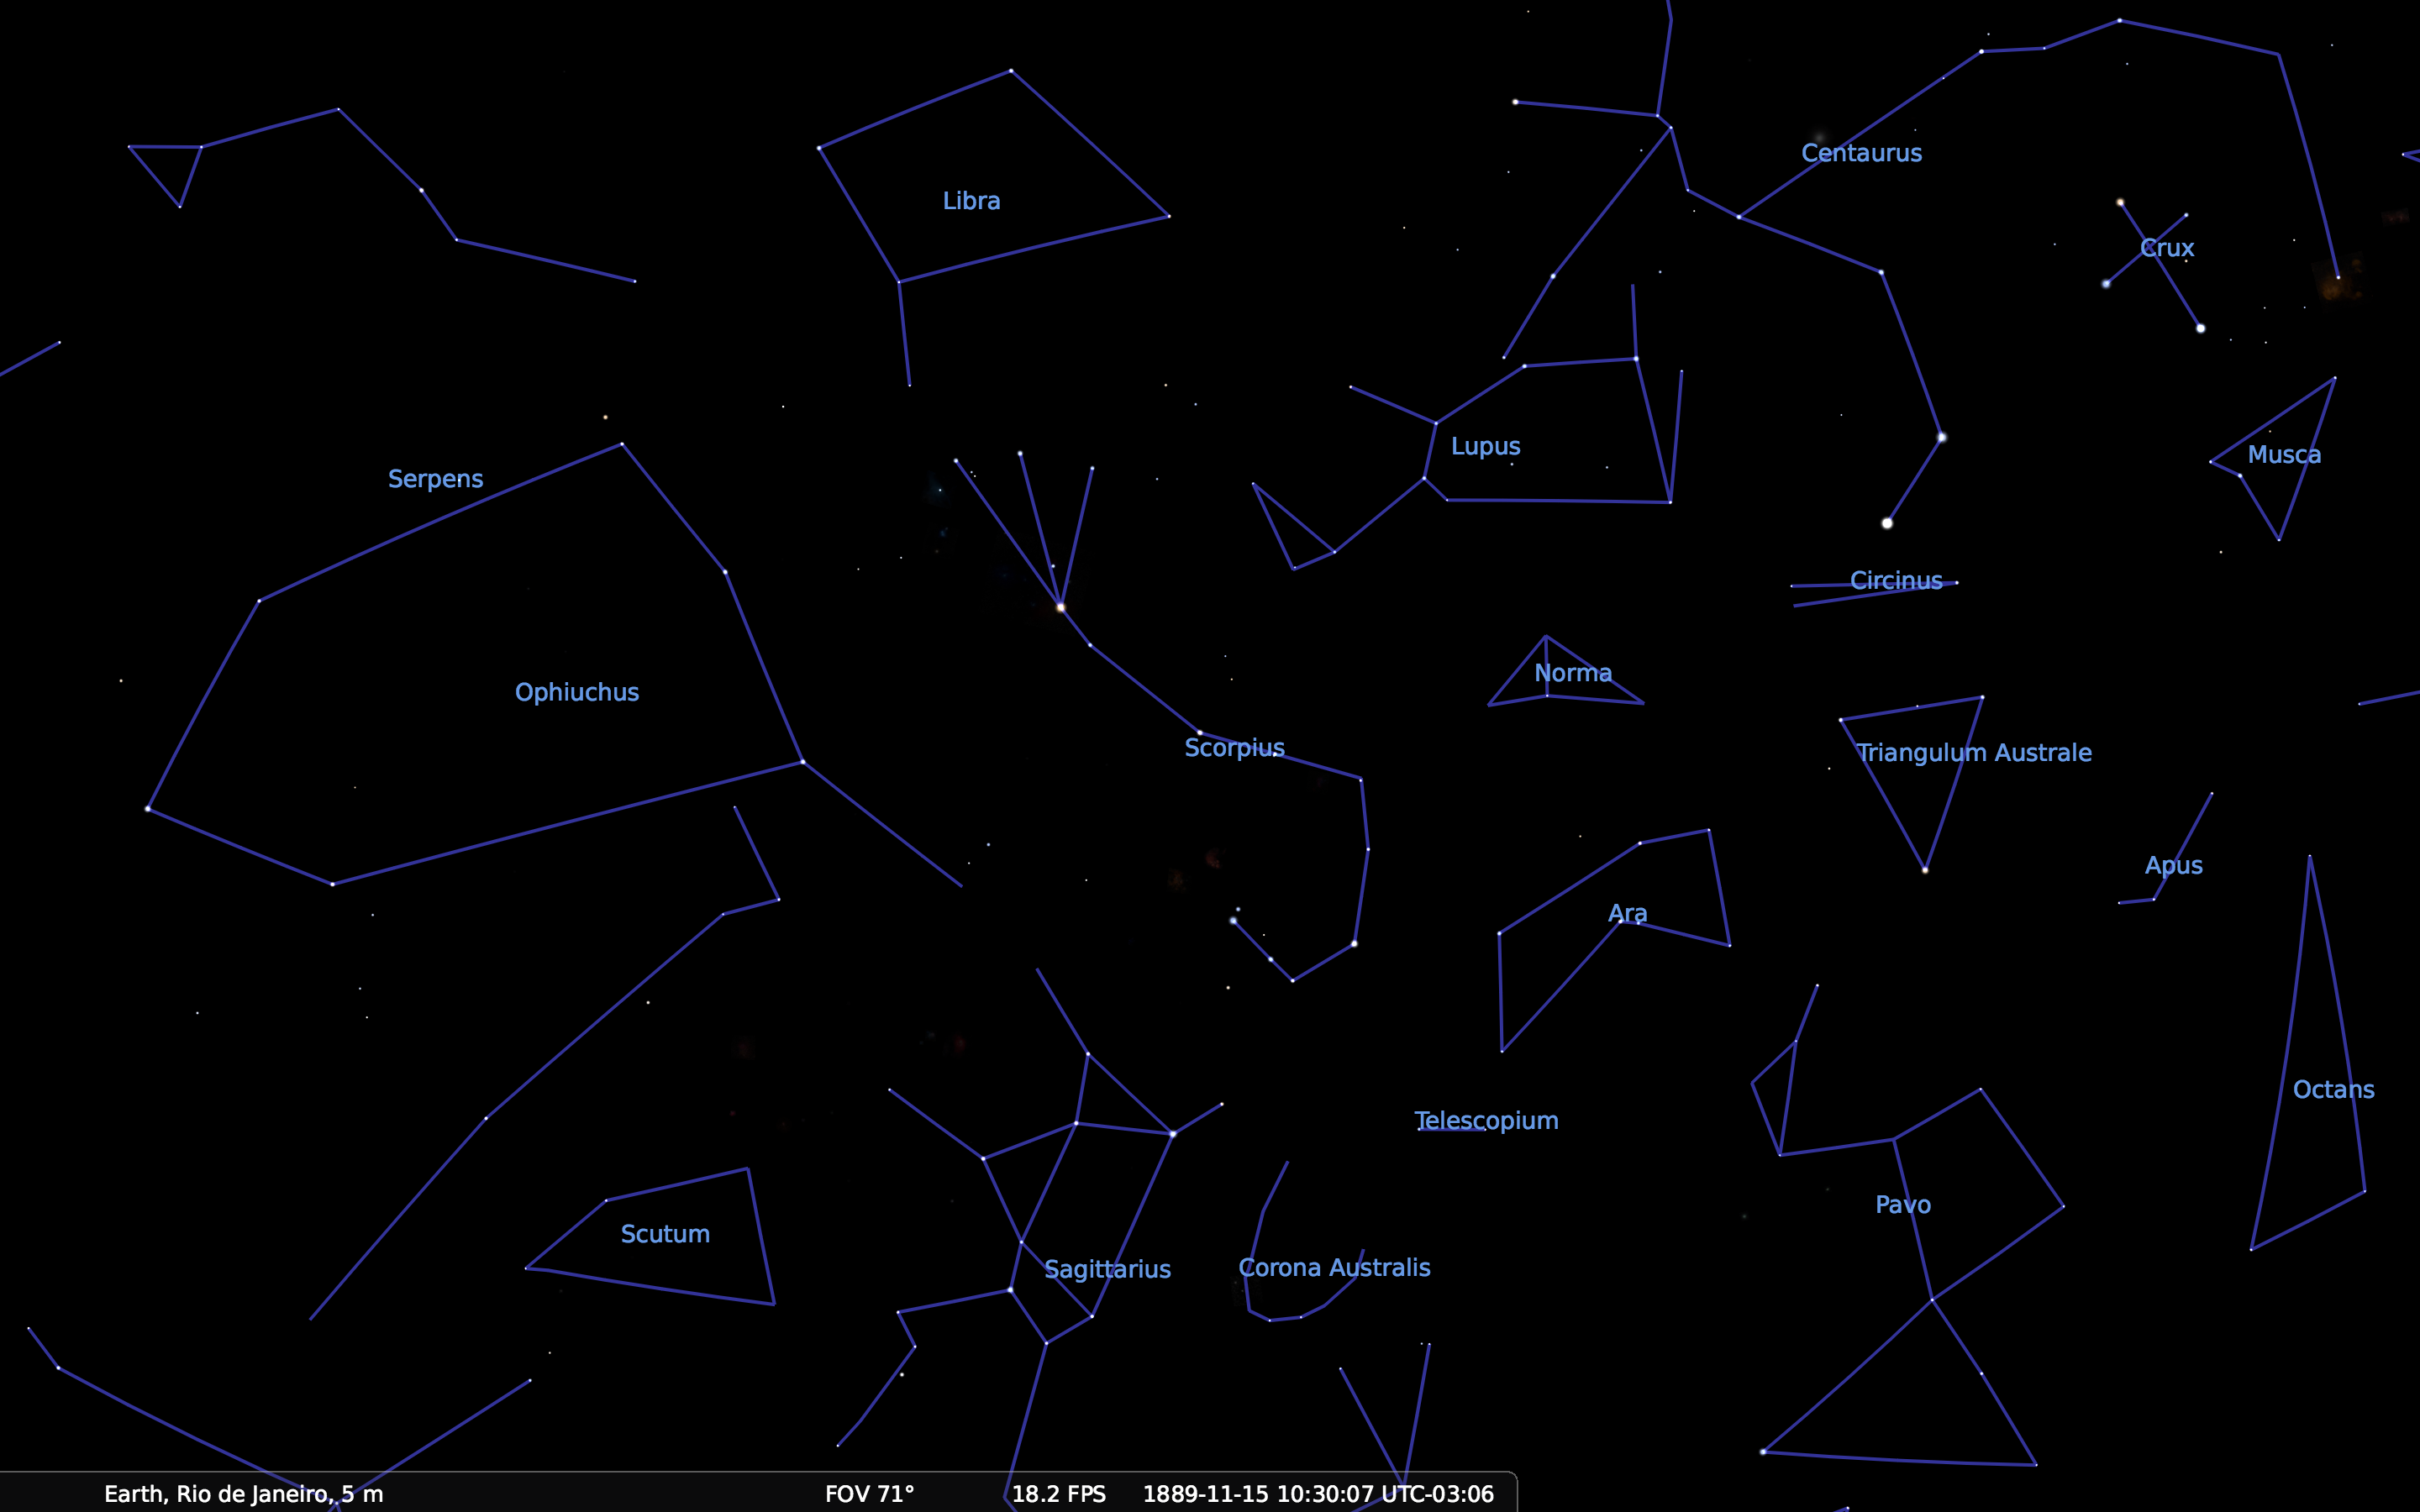
\includegraphics[width=1\columnwidth]{WesternCrux}
	\caption{Constellations displayed in Western sky lore.}
	\label{fig:WesternCrux}
\end{figure}

\begin{figure}[htbp]
	\centering
	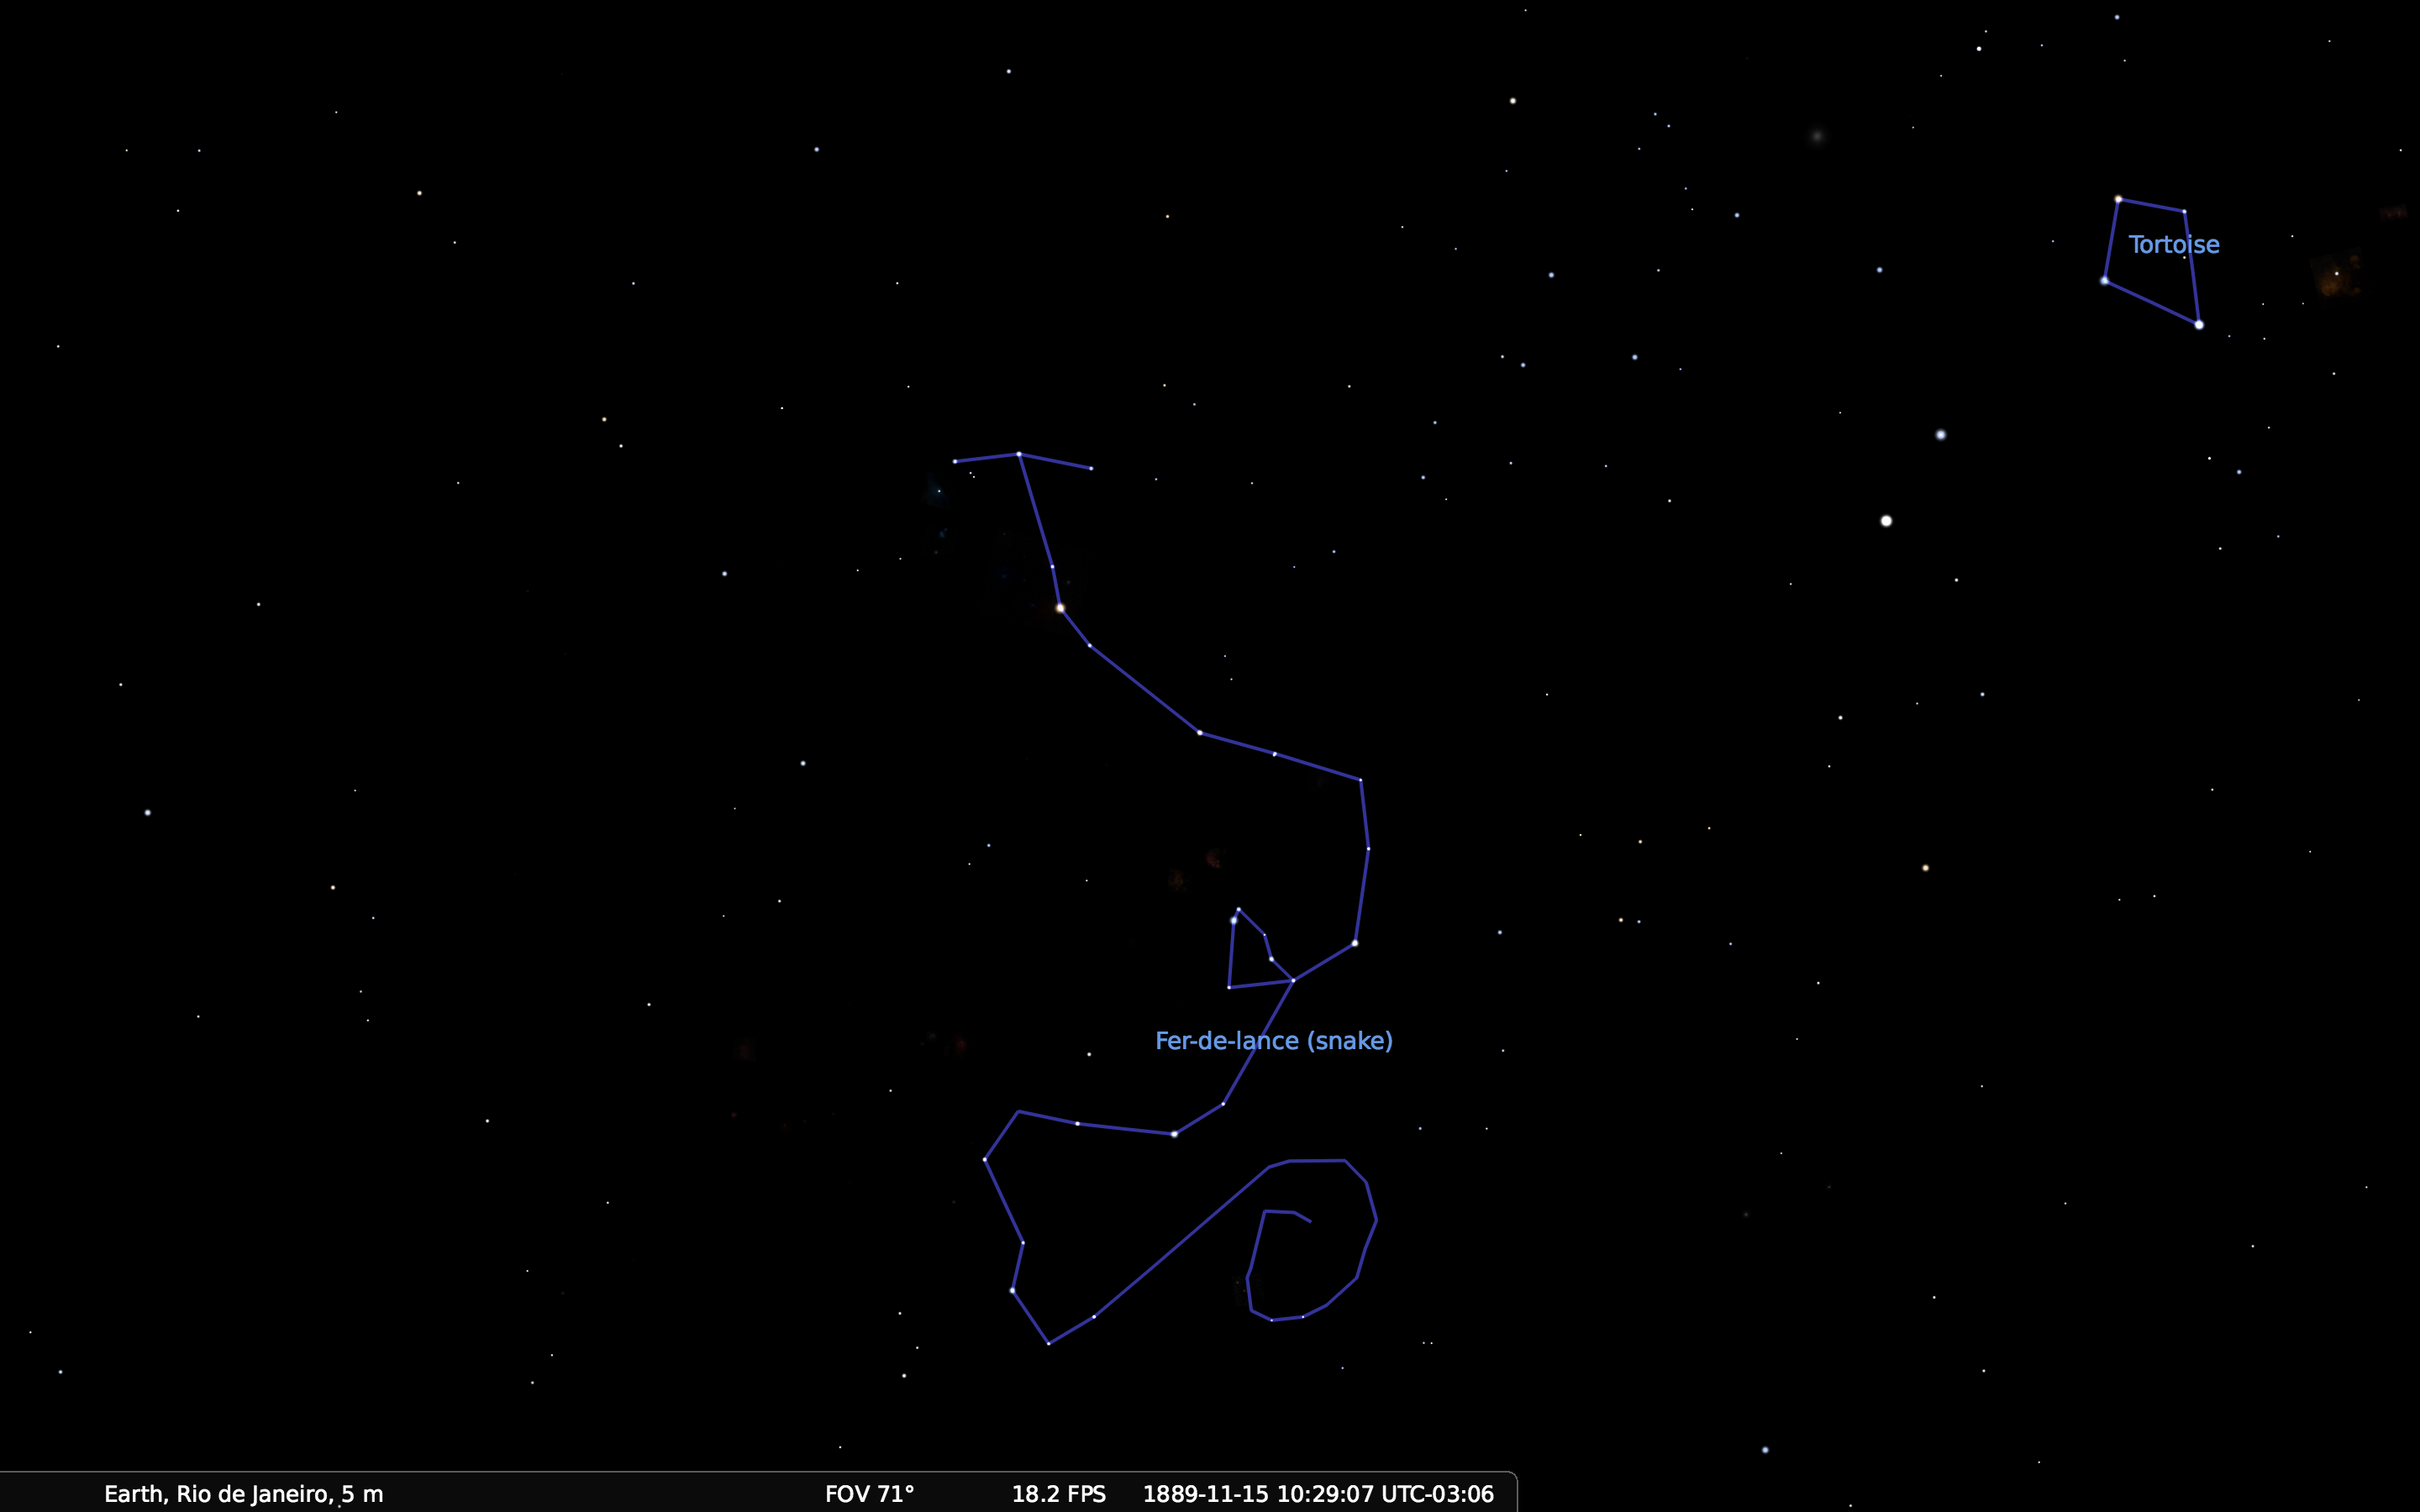
\includegraphics[width=1\columnwidth]{TukanoTortoise}
	\caption{Constellations displayed in Tukano sky lore.}
	\label{fig:TukanoTortoise}
\end{figure}

Many astronomers use Stellarium to display a prediction of the sky for a future time, such as organising a viewing night or planning an astro-photography session \cite{ashley2015computers}. Archaeoastronomers  also use the feature to generate an astronomical display from a location for a period sometime in the past \cite{zotti2014towards}. Also, the landscape feature facilitates a connection between  landscape and  skyscape, so one can map the sky against a landscape for research or aesthetics \cite{zotti2017skyscape}.

Stellarium scripts are written in ECMAScript, also known as Javascript, and enables the programmer to generate and run an automated astronomy presentation, facilitating  automation of all the functionality of Stellarium  \cite{zottistellarium}. 

Stellarium has a Remote Control plugin that enables third party programs to communicate with Stellarium via a REST client. This feature was used by the author to create an interactive spacecraft game using a sonic ball as a preliminary test of Stellarium's viability as a responsive performance interface \cite{fraiettaLAC2019}. The plugin also allows clients to query the status of Stellarium, including the area of sky currently being displayed.  The exact celestial vector and field of view displayed are used as the input to the VizieR server in order to obtain data about stars in that location.

\section{VizieR}
VizieR is an online database of high quality astronomical catalogues collected by the Centre de Donn\'ees astronomiques de Strasbourg (CDS), one of whose main goals  ``is to promote the usage of the reliable astronomical catalogues to the astronomical community" \cite[p.~25]{ochsenbein2000vizier}. One of the ways CDS ensures the reliability of their archives and catalogues is to only collect data that has been published or accepted in refereed scientific journals or literature. The number of catalogues available has grown from 3000 in 1999  \cite[p.~24]{ochsenbein2000vizier} to currently 18000 \cite{VizierPage}. Catalogues can be selected by name or based on the wavelength, mission and astronomy type \cite{vizquery}.  Wavelength dictates the frequency spectrum of the data in the catalogue, such as radio, infra-red, optical, x-ray, and Gamma-RAY. The mission indicates the purpose for which the catalogue was created or is used. For example, the purpose of the Kepler Mission is to ``detect Earth-size planets in the habitable zone ... of solar-like stars... , determine their frequency, and identify their characteristics." \cite[p.~2]{koch2010kepler}; and so catalogues created or used within this mission can be specifically targeted. The type of astronomy indicates the subject area of research that the catalogue belongs to; for example,  black holes, galaxy clusters, planetary nebulae, red shifts, and photometry. 

Once a user has selected the database criteria to search, they must provide VizieR  a search window that consists of a target centre and area around that point to search. The target centre is the point on the celestial sphere referenced to a celestial equinox\footnote{The default equinox is J2000 \cite{vizquery}.}, and can be defined by object name,  RA and Dec., or by IAU-coordinates \cite{vizquerytarget}.


\section{Stellar Command Module}
Although it is possible to communicate directly to Stellarium and VizieR directly through the HTTP interface, the stellar position parameters between the two systems are different. Stellarium returns its position information as three dimensional spherical points, with a separate query for the field of view; whereas, VizieR requires the data as a two dimensional geometric point with a defined radius. The Stellar Command module abstracts this information from the client software and removes the requirement to perform these calculations by the client. Stellar Command directs VizieR to query the Hipparcos catalogue because it provides a ``complete all-sky survey of astrometric and photometric parameters for one million stars down to magnitude 11 " \cite [p. ~201]{van1997hipparcos}. An attempt was made using other photometric catalogues, however, it was difficult to obtain consistent results for all sky locations.  

The interface required to control both Stellarium and VizieR was HTTP based, so a language that provided network functionality as a fundamental core feature was preferred. Also, it was imperative that third party users of the library should not have to learn a particular programming language, but instead, could easily interface with the library using their preferred music package such as Max MSP, SuperCollider or PD. Furthermore, it would be advantageous for users to be able to integrate the library  into the programming language of their choice, such as C, C++, Python, Ruby, or Java. 

Developing the system as a Java Archive (JAR) fulfilled all these requirements. Using a JAR file allowed instantiation from the command line, running as separate processes and using OSC to communicate with other programs. Additionally, many other programming languages can connect directly to a JAR through the Java Native Interface (JNI) \cite{liang1999java}. 


\chapter{Terminology}
In all areas of research or vocation, there is terminology used that is specific to that field, and astronomy is no exception. Although this is not a treatise on the study of astronomy, it would serve you well to become acquainted with some of these terms.

\section{Disciplines of research}

You will hear terms such as \textit{astronomy, archaeoastronomy} and \textit{ethnoastronomy}. These terms can sometime become confusing so I will provide short definitions for them.

\subsection{Astronomy}
Astronomy is one of physical sciences and involves the systematic study of celestial objects and phenomena that originate outside the Earth's atmosphere. Astronomic data from various missions are recorded in catalogues for use within the scientific community. Within the field of study, there are various terms used, which are important to know in order to query and interpret the astronomical data you will encounter.

\subsubsection{Field of View}
The \textit{field of view} is the amount of sky that you are able to see and it is measured in degrees.  If we zoom in, we reduce the field of view. If we compare Figures~\ref{fig:fov60} and ~\ref{fig:fov13}, we see the same point of sky is in the centre, however, the image that looks closer has a lower field of view.

\begin{figure}[htbp]
	\centering
	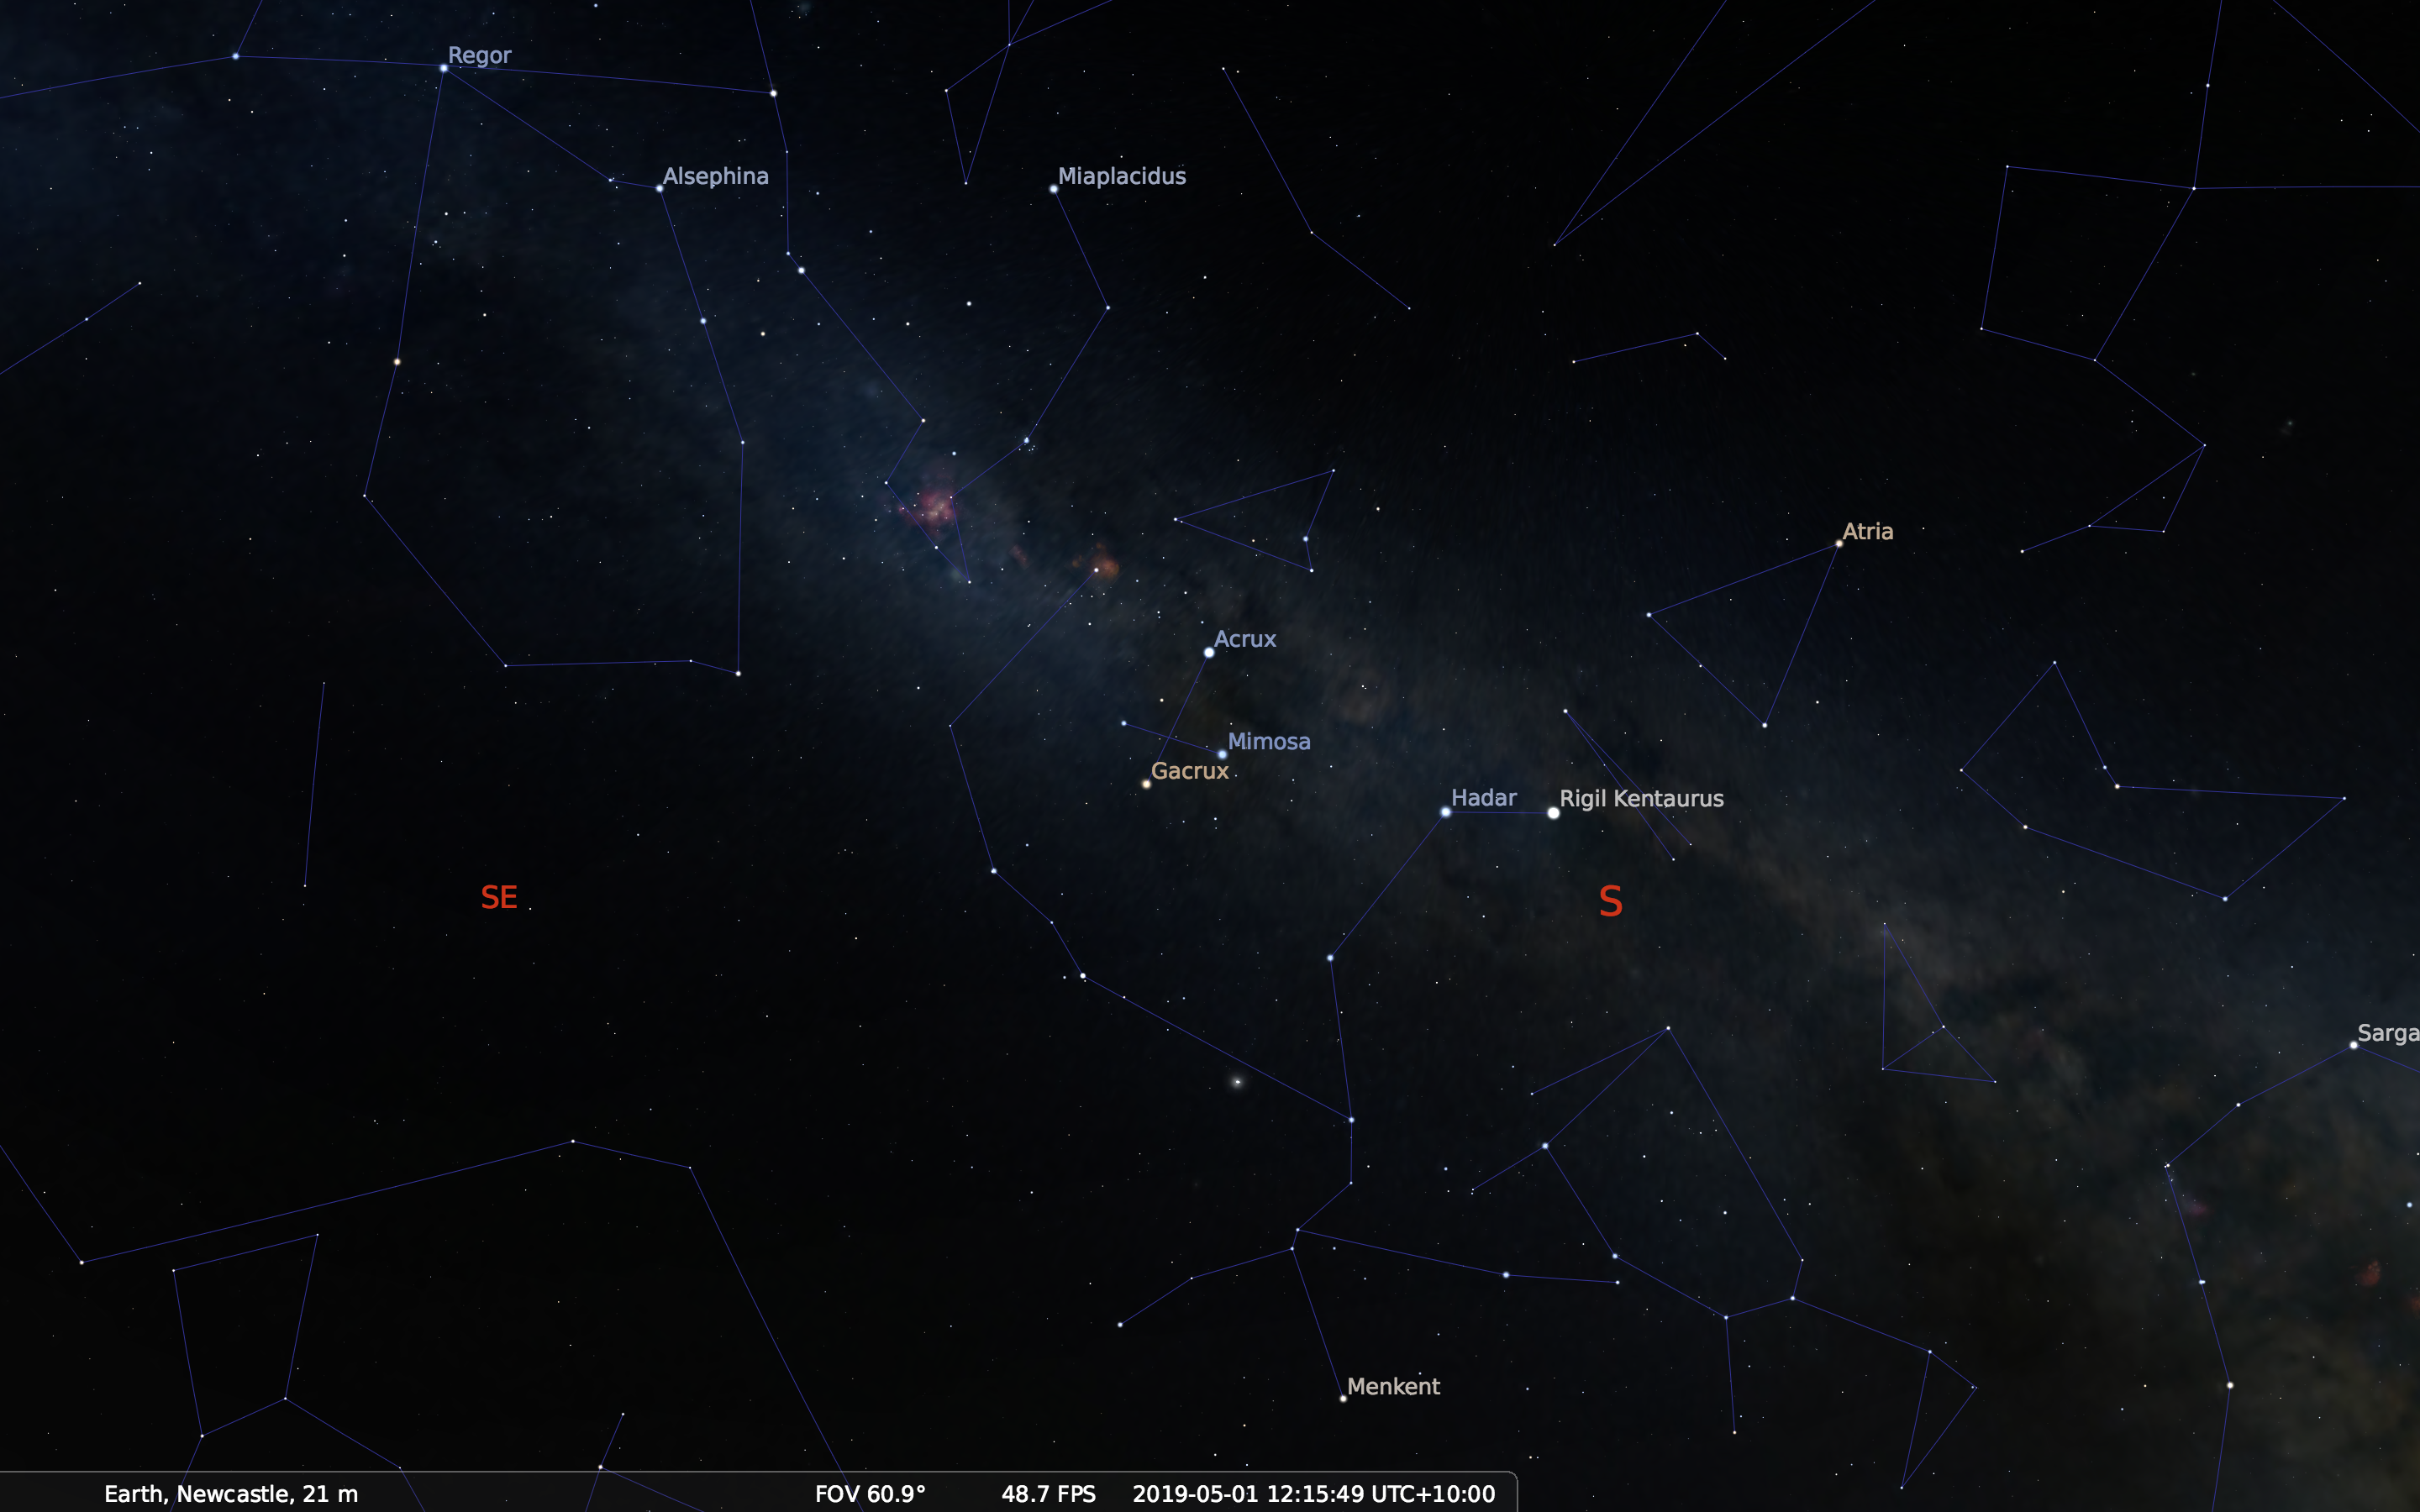
\includegraphics[width=1\columnwidth]{fov60}
	\caption{Stellarium displaying a 60$^{\circ}$ field of view.}
	\label{fig:fov60}
\end{figure}

\begin{figure}[htbp]
	\centering
	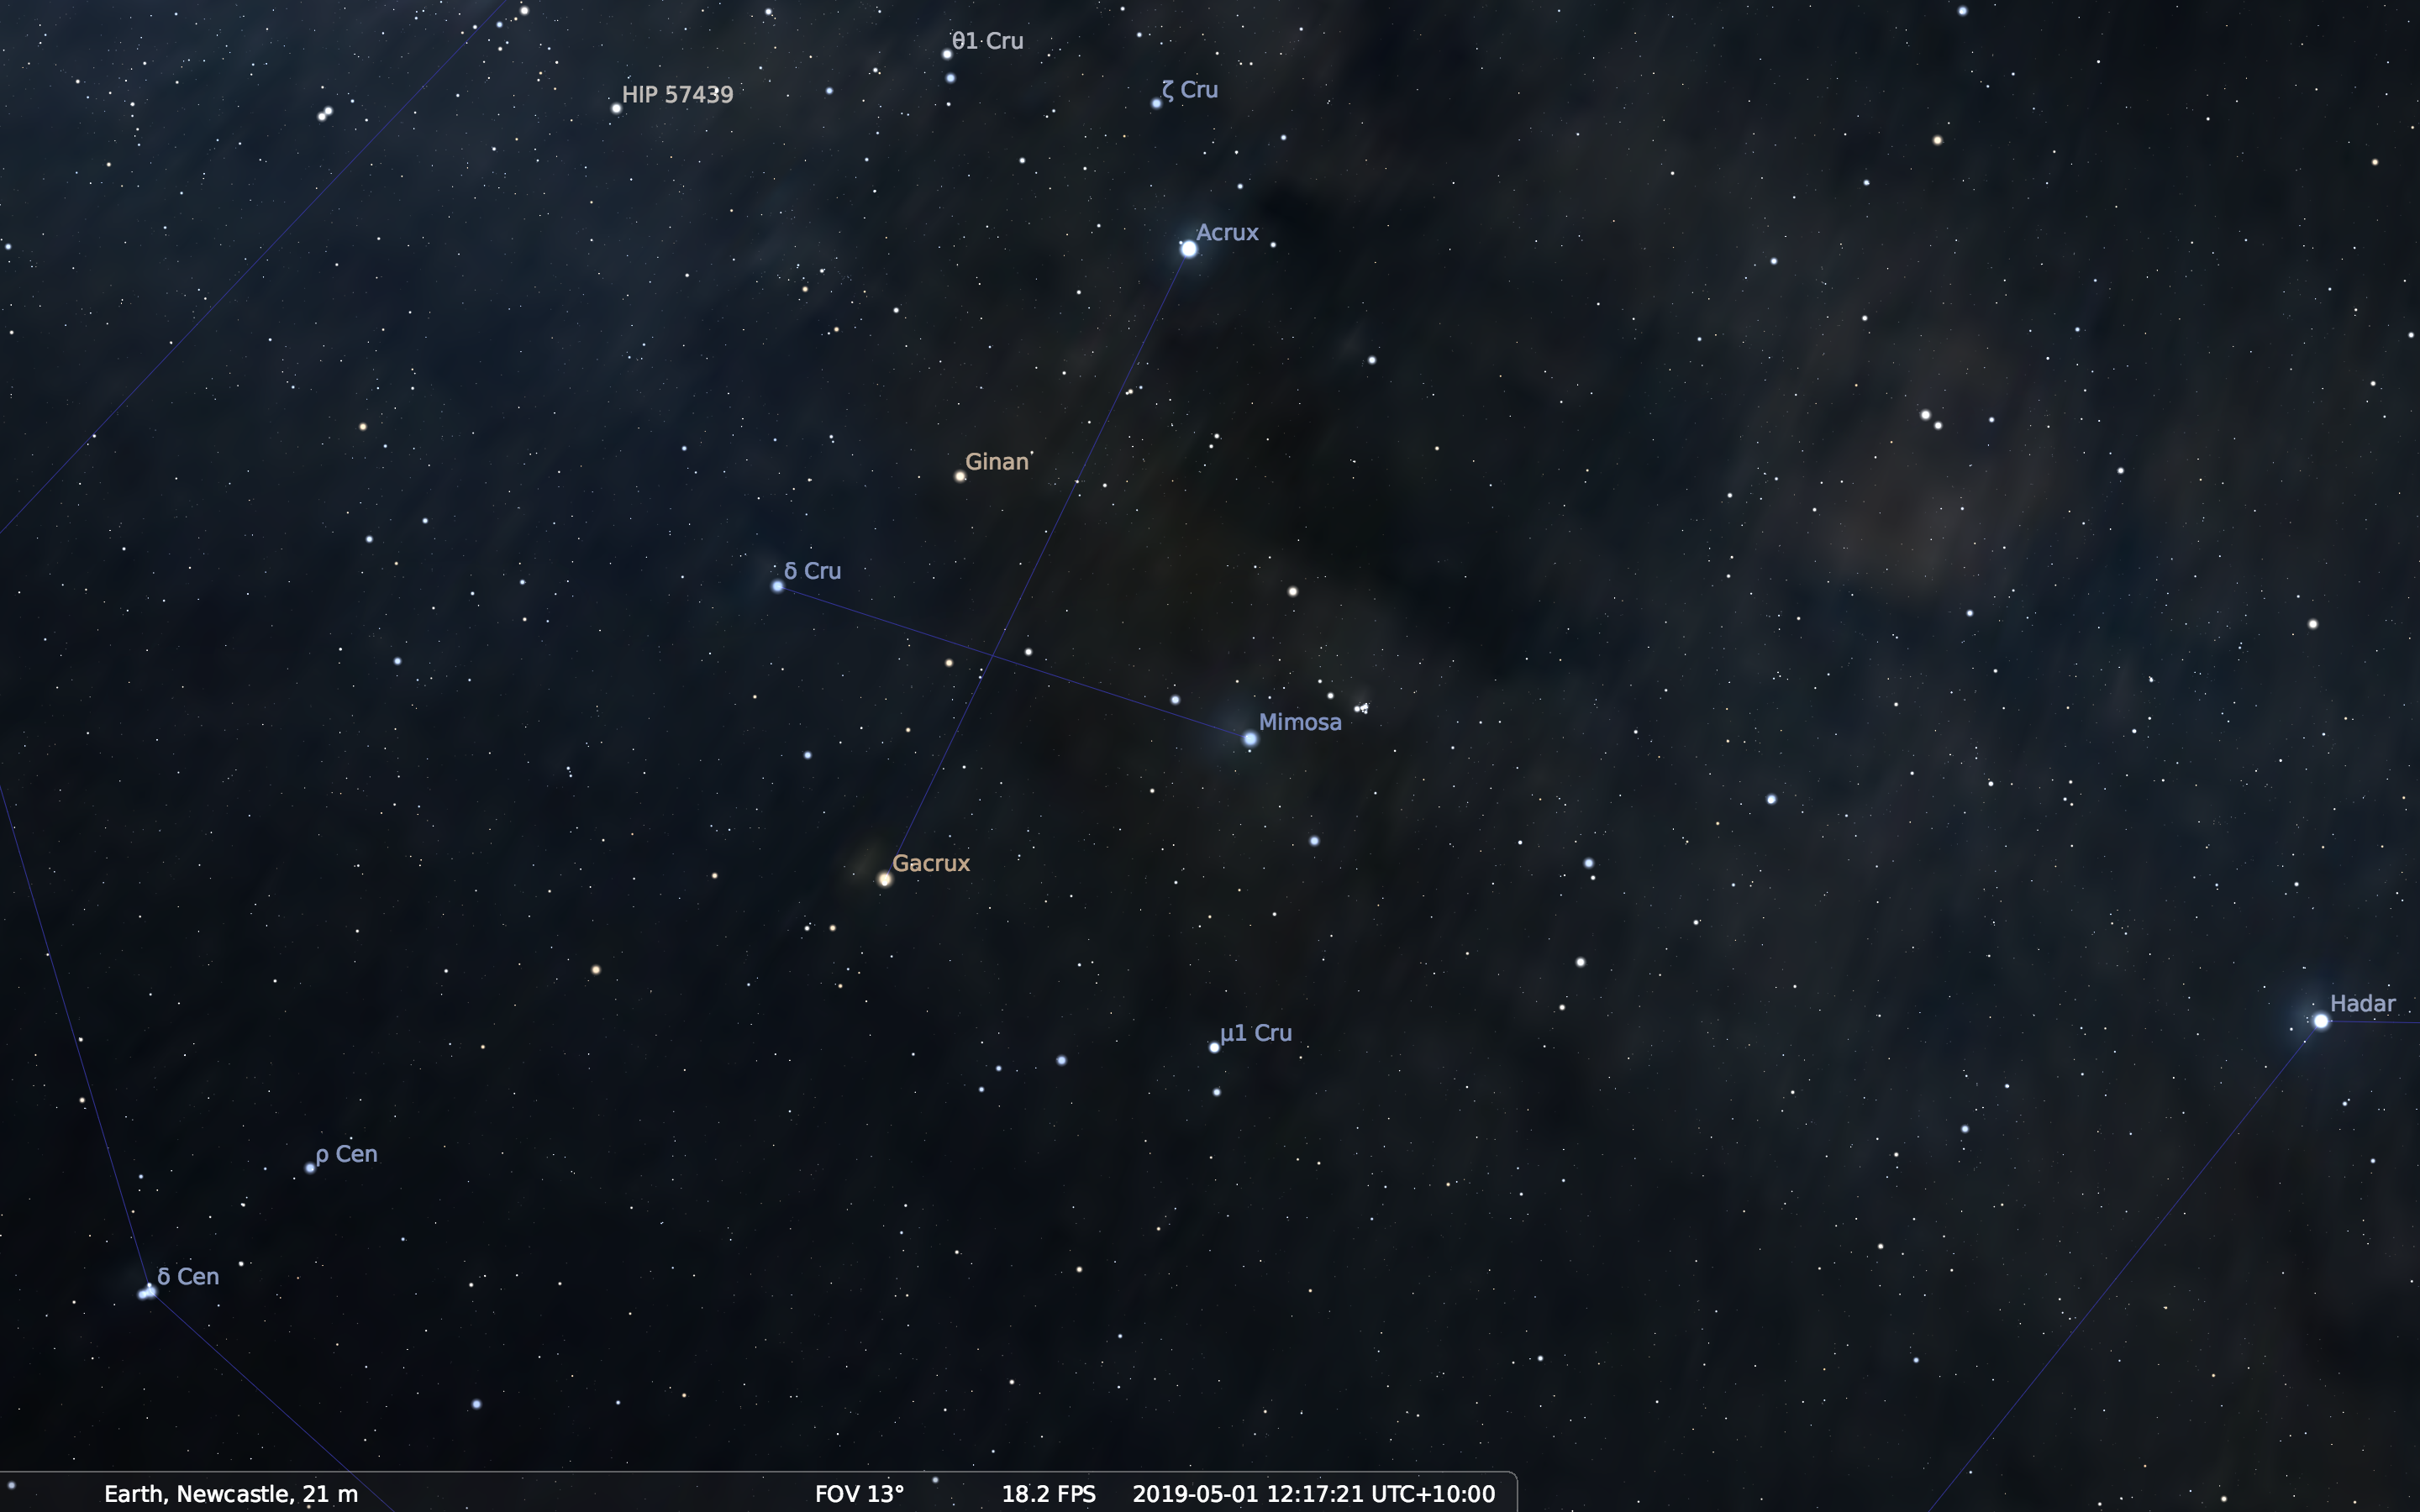
\includegraphics[width=1\columnwidth]{fov13}
	\caption{Stellarium displaying a 13$^{\circ}$ field of view.}
	\label{fig:fov13}
\end{figure}

\subsubsection{Observation Location}
The observer location is the geographical position from where the celestial observation is being made. These are defined using latitude and longitude. For example, if you were viewing the sky from Newcastle Australia, your geographical location would be  32.9283$^{\circ}$ South, 151.7817$^{\circ}$ East. Rather than using the terms south and east, northern latitudes are positive and southern are negative. Likewise, east is positive and west is negative. Therefore, the geographical location for Newcastle would be -32.9283, +151.7817.  A western longitude can also be positive, however, the value is 360$^{\circ}$ - the western longitude. Eg, a longitude of -90$^{\circ}$ is also +270$^{\circ}$.

It is also possible to set the planet or celestial body you are viewing from. 
For example, Figure ~\ref{fig_JupiterFromIO} displays us looking at Jupiter with our observation location as its moon Io.

\begin{figure}[ht]
	\centerline{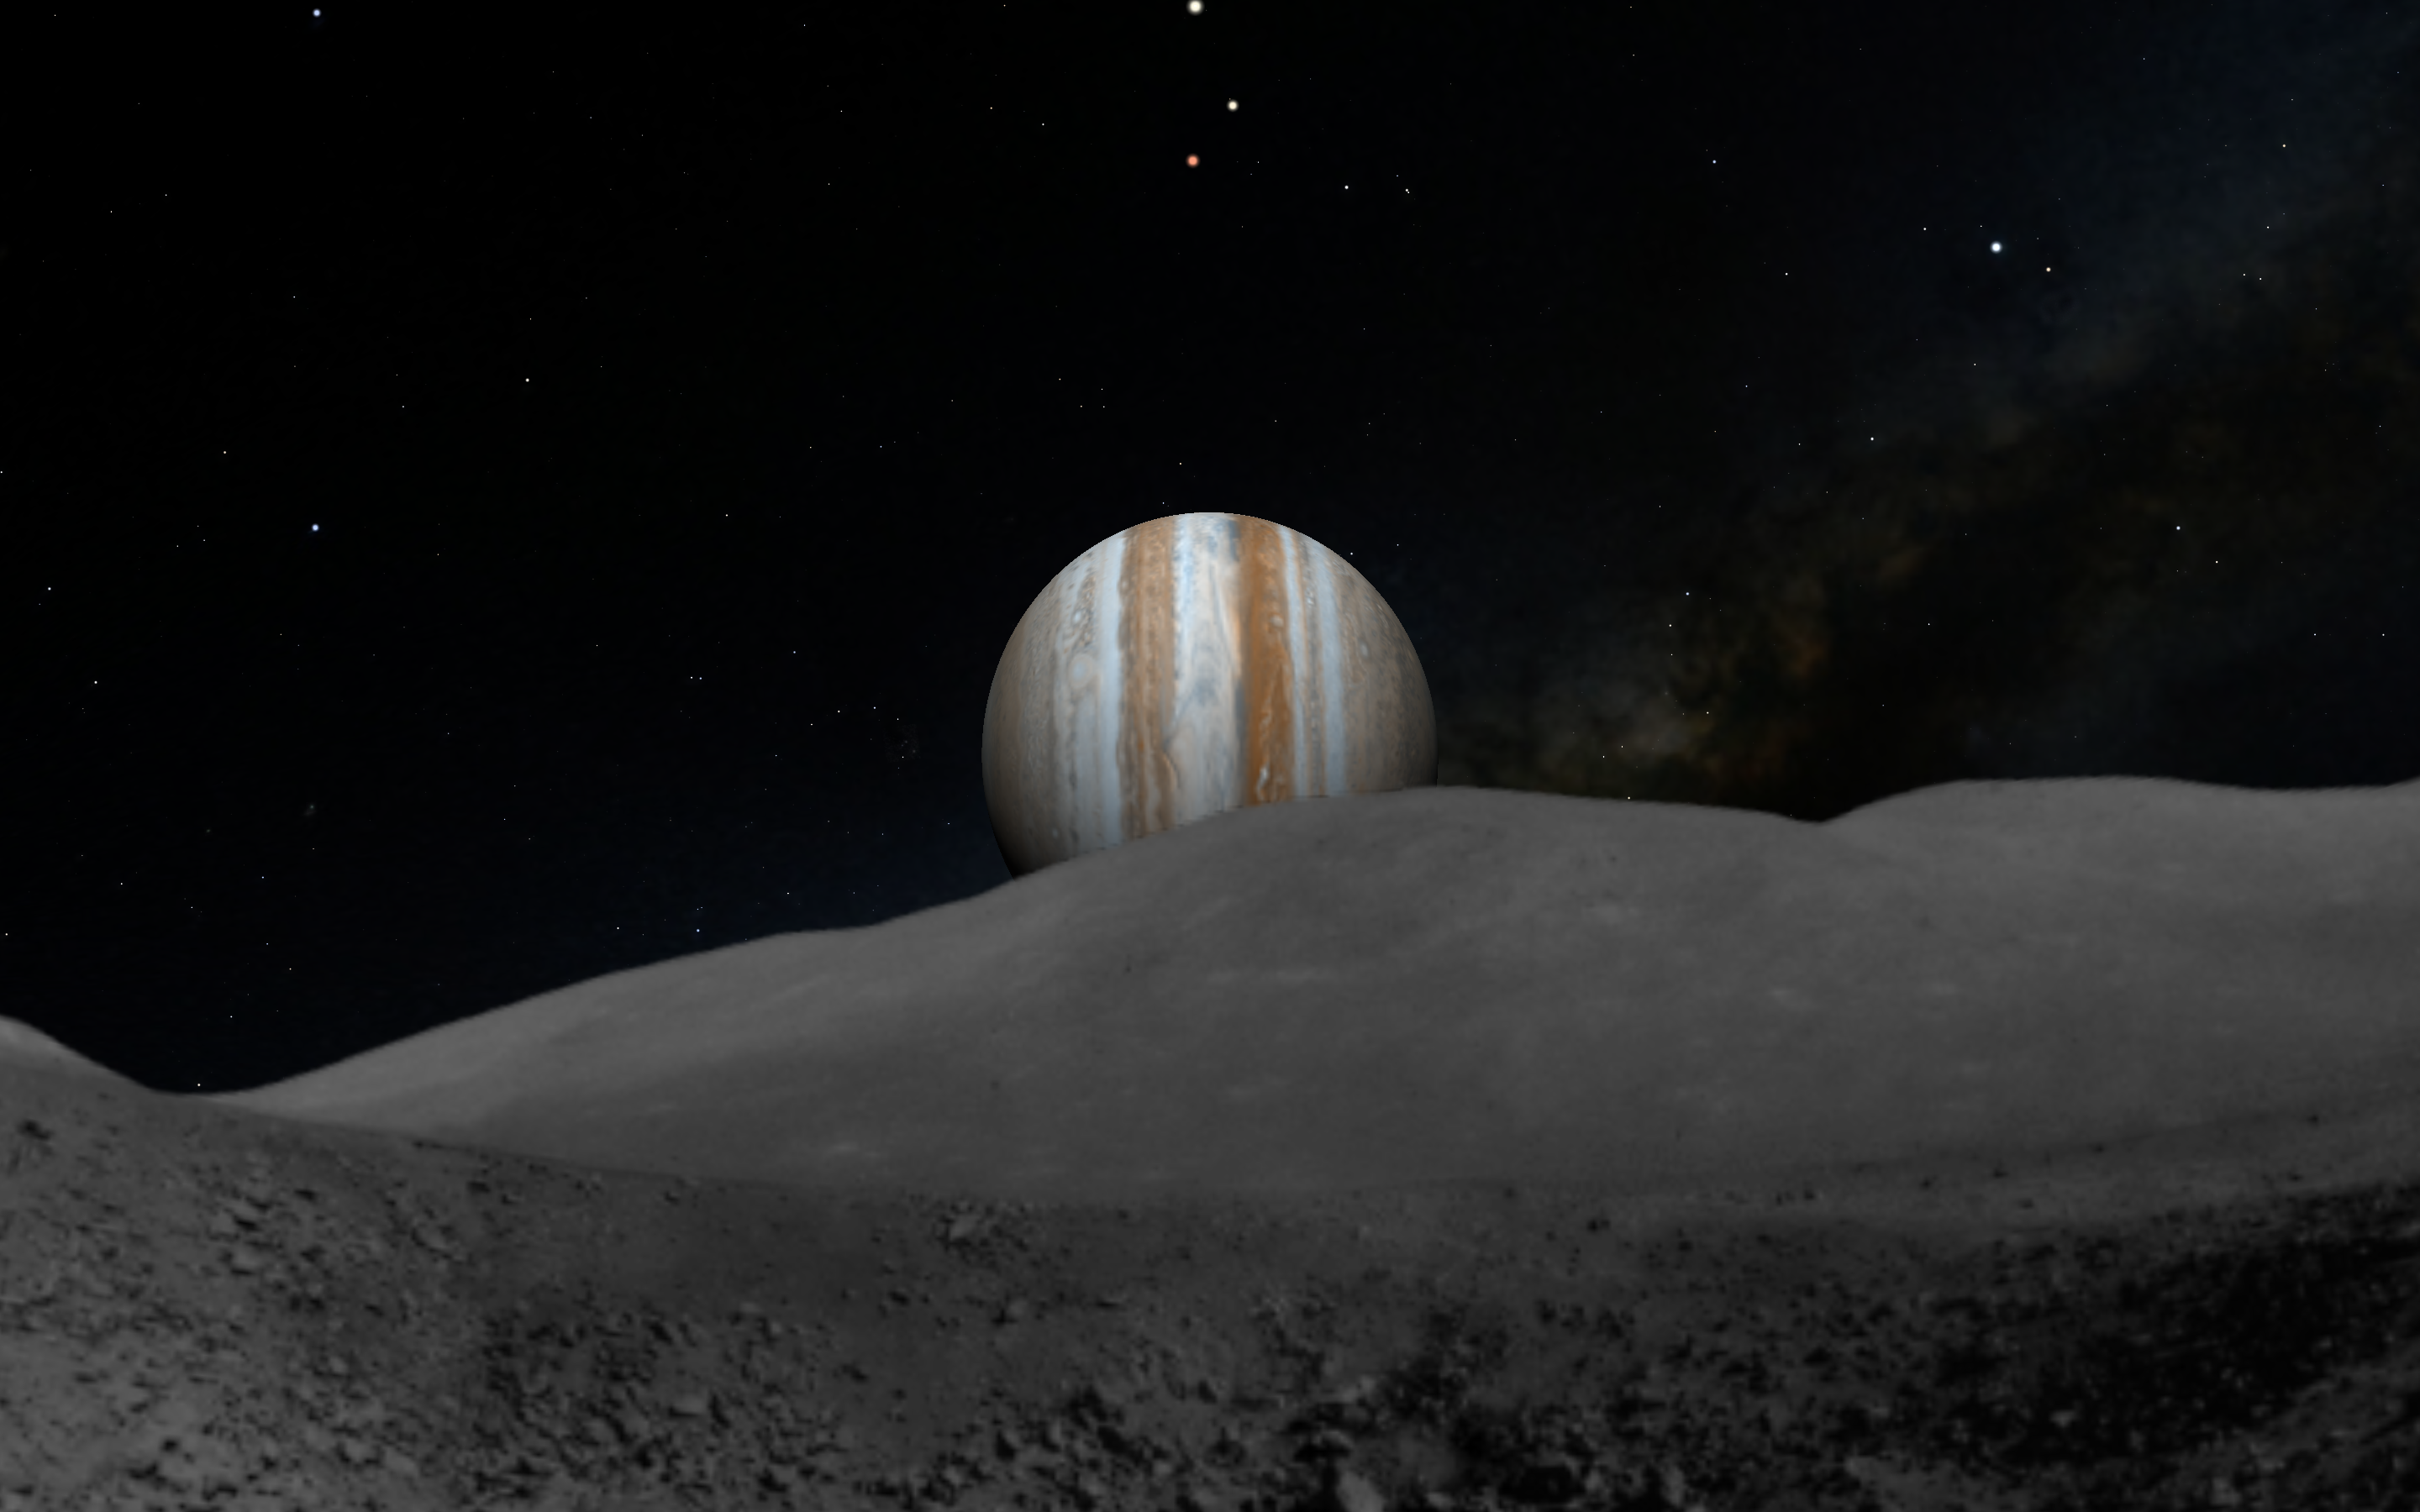
\includegraphics[width=1\columnwidth]{JupiterFromIO.png}}
	\caption{\label{fig_JupiterFromIO}{A simulation of Jupiter being viewed with Io as the observation location.}}
\end{figure}

\subsubsection{Time Zone}
The time zone is the time difference between local time and Coordinated Universal Time (UTC) and does not change with daylight saving. The exact time is specified by the year, month, day followed by time in hours (24 hour code), minutes, seconds and the time zone.  The time zone for UTC is "Z", witch each hour time zone increasing by a letter of the alphabet, with "Z" being zero. For example,   midday on January 1, 2000 at UTC would be defined as "2000-01-01T12:00:00Z". Likewise, "2019-06-01T14:13:00K" would be 1 June 2019 at 2:15pm, 10 hours later than UTC time (this is Sydney time). When daylight saving occurs, the local time changes, which results in a different letter for the time zone.


\subsubsection{Celestial Coordinates}
In the same way we can define an exact location on the Earth using latitude and longitude, we define the location of celestial objects using the celestial coordinate system. Instead of longitude and latitude, we use the terms \textit{Right ascension} and \textit{Declination}. 

\subsubsection{Right Ascension}
Right Ascension, abbreviated to \textit{RA}, is the angular distance from the east of the First Point of Aries (hereafter FPOA), and is measured in hours, minutes and seconds, and is similar to the longitude on earth, except on the celestial sphere. This is basically how long it takes from the time FPOA is on the meridian (directly north or south) for the RA in question to be overhead. For example, if an object had a Right ascension of 3 Hours, it would mean that it would appear on the meridian three hours after FPOA was.  This is similar to the concept of time zones. In order to make calculations easier, we convert the RA to a digital angle by multiplying the number of hours by 15 (24 hours x 15 = 360$^{\circ}$) . Furthermore, we use decimals instead of minutes and seconds. eg, 90$^{\circ}$ 30' would be written 90.5$^{\circ}$. 

\subsubsection{Declination}
The declination is equivalent to the concept of latitude and is the angular distance a star is north or south of the celestial equator when it is on the meridian (in line with north / south).  

\subsection{Magnitude}
The magnitude is how bright a star is. Higher magnitudes mean a lower brightness.

\subsection{Atmosphere}
Atmosphere is the gas that surrounds us and makes the sky appear like daylight. If there was no atmosphere, the sky would appear dark, as it does on the moon, and you would be easily able to see stars during the day. Stellarium gives us the option to hide the atmosphere, enabling us to see stars at any time. For example, Figure ~\ref{fig_with-atmosphere} shows the midday with normal atmosphere, whereas ~\ref{fig_no-atmosphere} shows the same sky without the atmosphere.

\begin{figure}[ht]
	\centerline{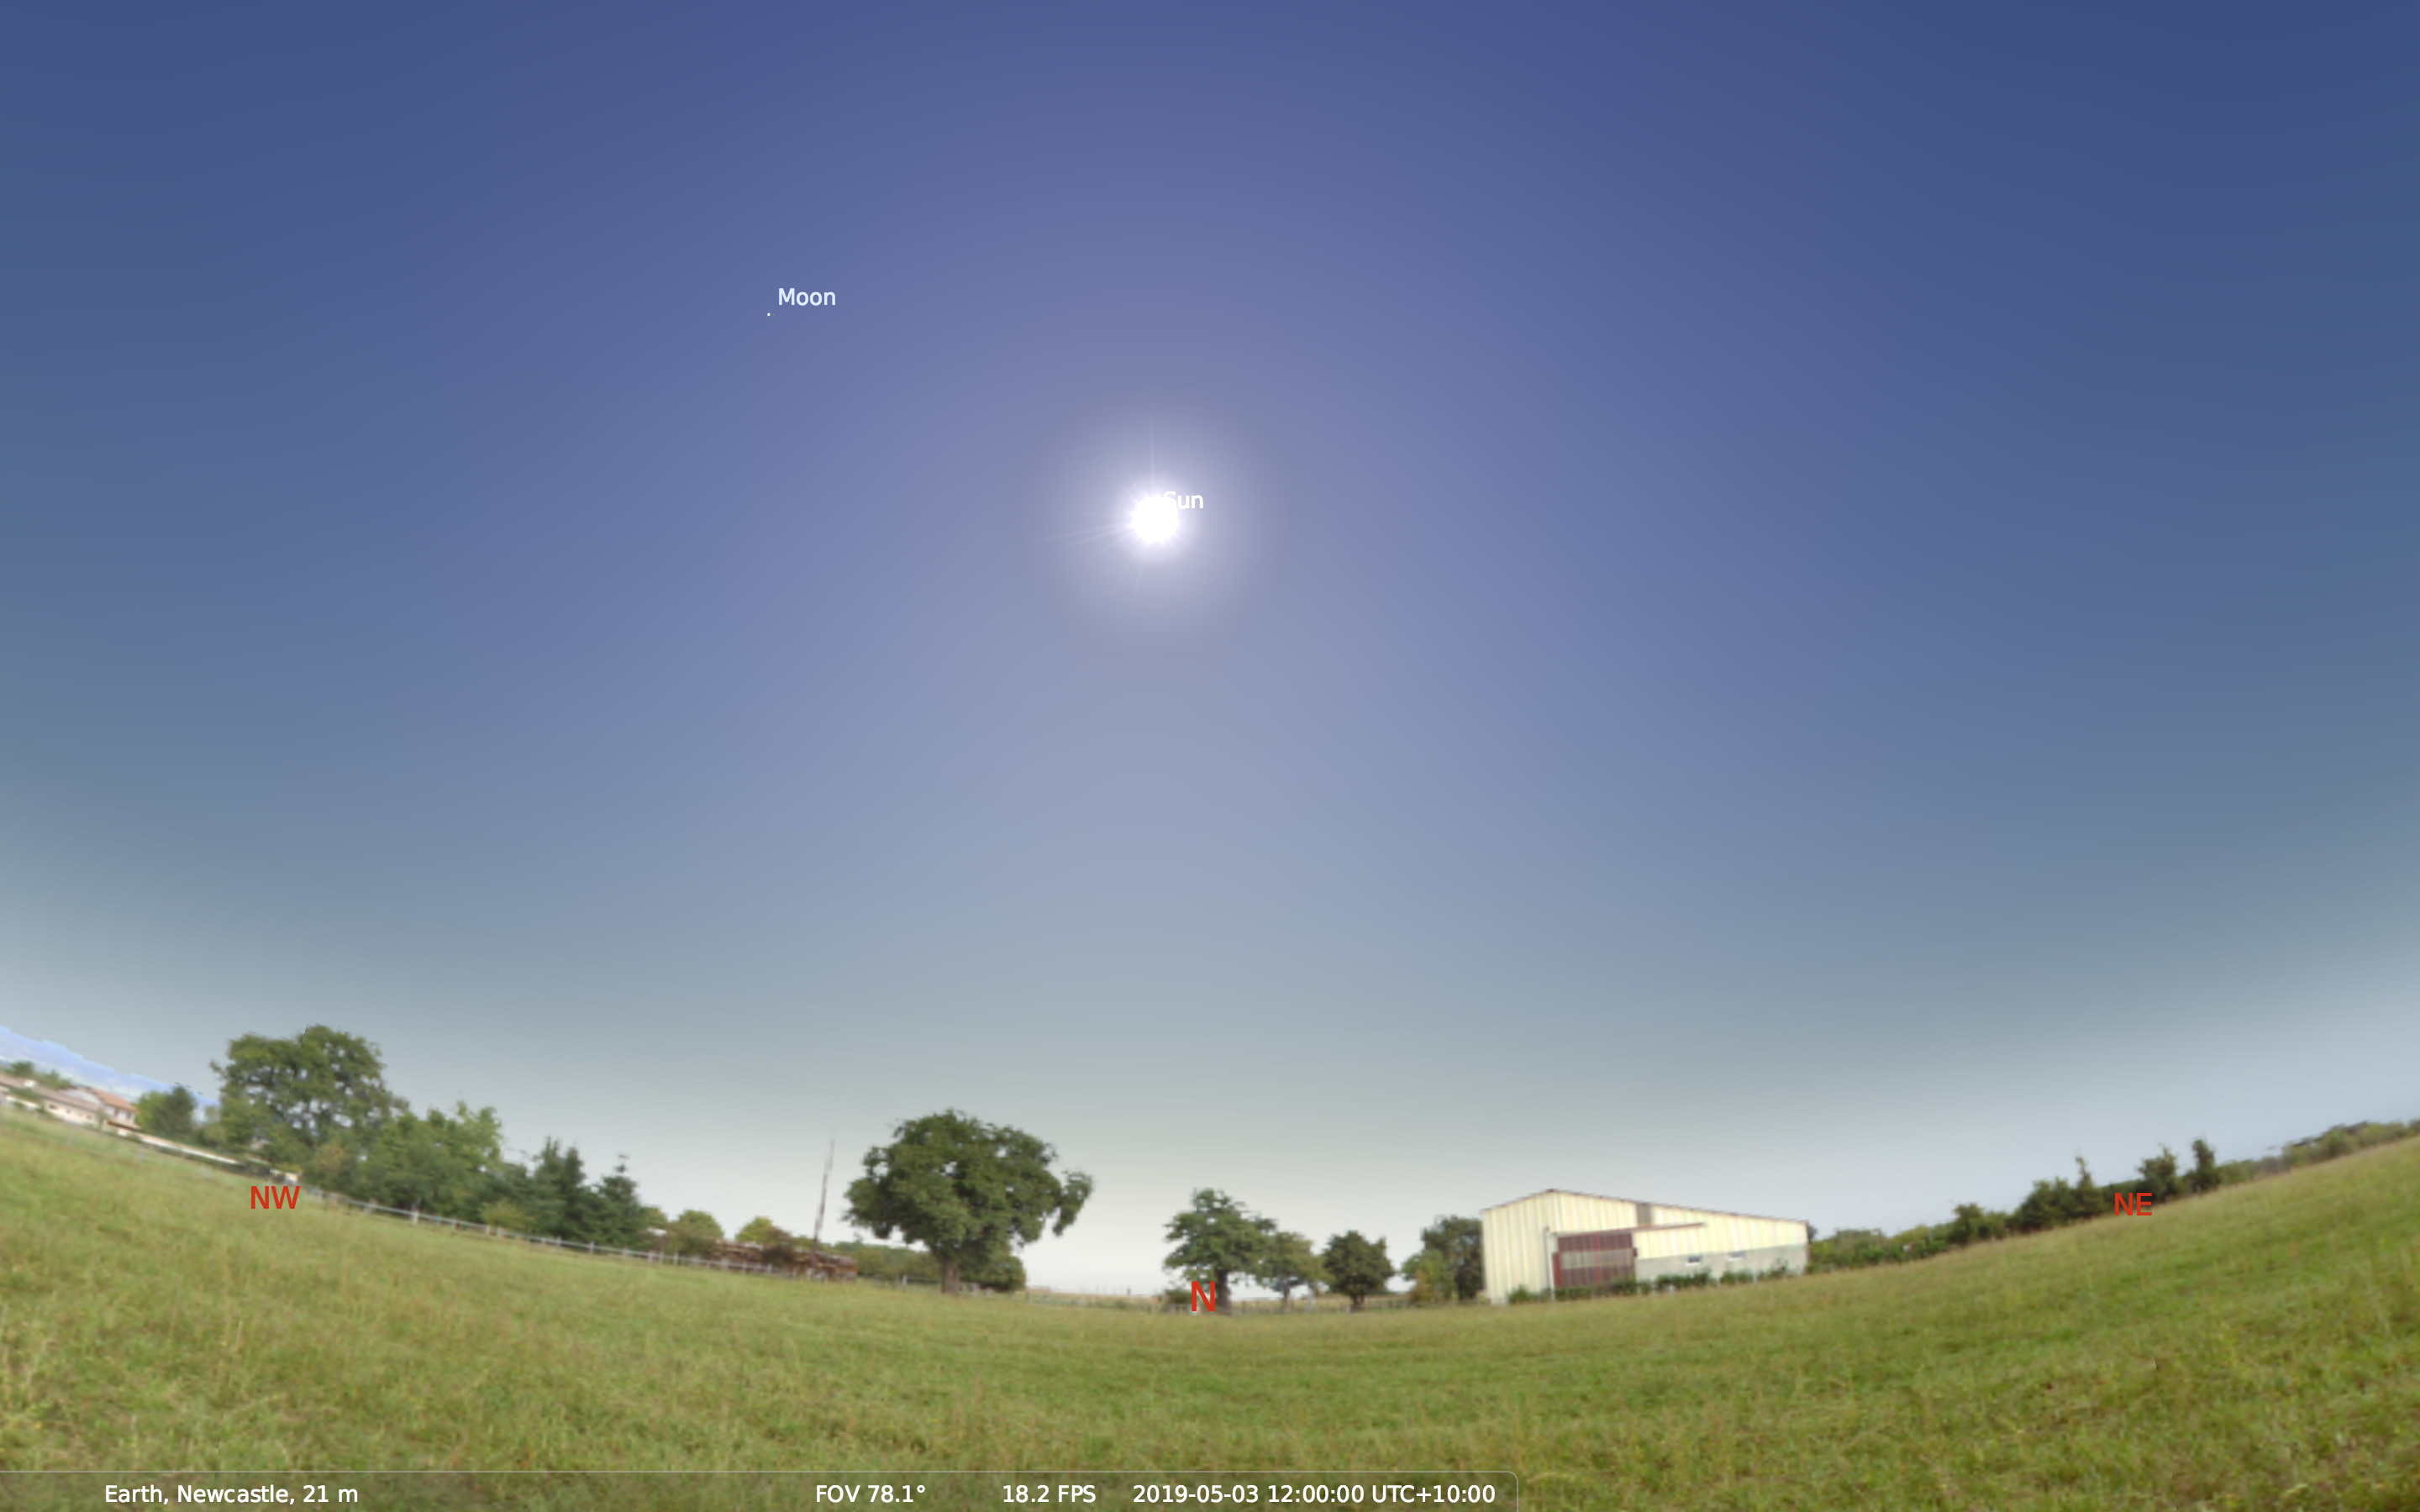
\includegraphics[width=1\columnwidth]{with-atmosphere.png}}
	\caption{\label{fig_with-atmosphere}{Midday showing the sky with atmosphere.}}
\end{figure}

\begin{figure}[ht]
	\centerline{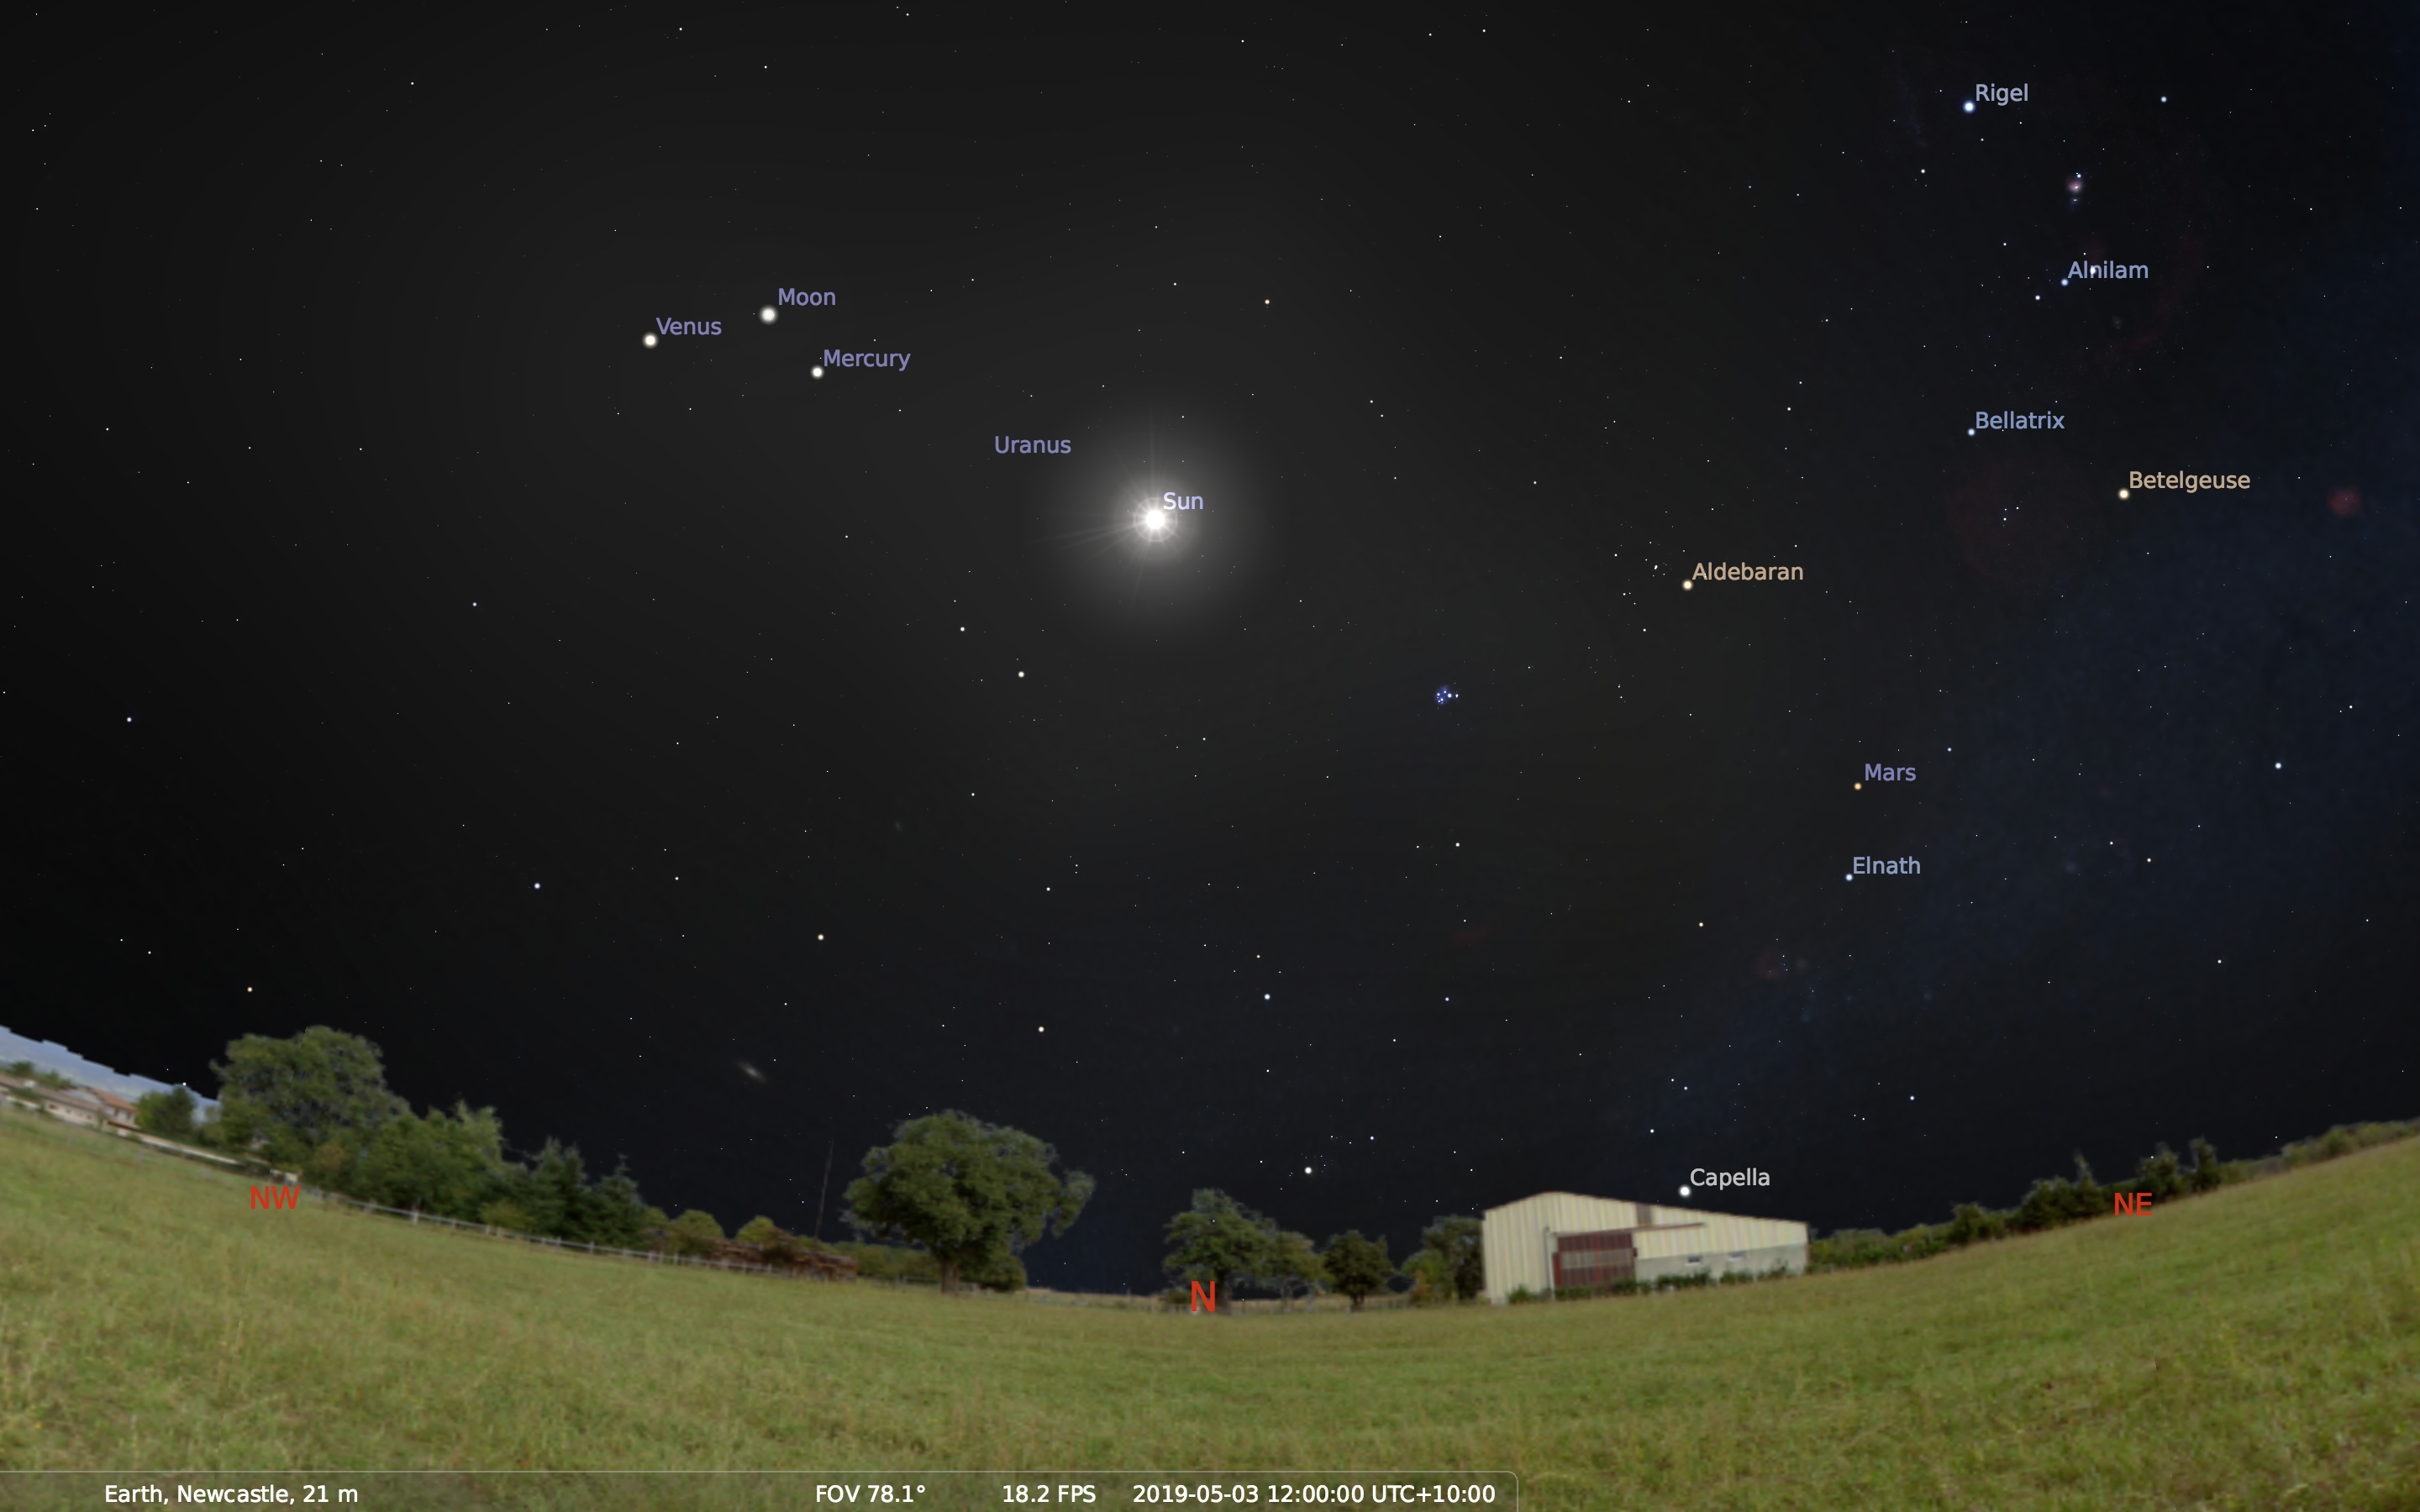
\includegraphics[width=1\columnwidth]{no-atmosphere.png}}
	\caption{\label{fig_no-atmosphere}{Midday showing the sky with atmosphere.}}
\end{figure}


\subsection{Ethnoastronomy}
Ethnoastronomy is a social science belonging to the discipline of ethnology and examines the way astronomy is practised in the context of a particular culture \cite{Salt2015}.

\subsection{Archaeoastronomy}
Archaeoastronomy is the study of how ancient civilisations understood the cosmos and in a sense very similar to ethnoastronomy.
``Broad public embrace of archaic astronomy probably began in the eighteenth
century with awareness of the summer solstice sunrise’s affiliation with Stonehenge" \cite[p.~263]{Krupp2015}.
Archaeoastronomers have used Stellarium to generate an astronomical display from a location for a period sometime in the past \cite{zotti2014towards}. 

\subsection{Astrology}
``Astrology, from the Greek, astro-logos, is the assumption that the stars and planets
contain meaning and significance for terrestrial affairs....Astrology appears to
be a universal feature of human culture and may be understood as a form of cultural
astronomy; an important contribution to the understanding of astronomy’s cultural
uses, applications, uses, and functions; and an indication of society’s attitudes to the
stars."\cite[p.~104]{Campion2015}. Stellarium has a feature whereby you can display constellation art, as shown in ~\ref{fig_constellation-art}, which facilitates representing astrology in your works. 

\begin{figure}[ht]
	\centerline{\includegraphics[width=1\columnwidth]{constellation-art}}
	\caption{\label{fig_constellation-art}{Constellation art.}}
\end{figure}


	



\mainmatter

\pagenumbering{arabic}

\chapter{Installing Stellar Command} \label{chap:install}
Installing Stellar Command is completed in two parts: the Stellar Command module and the examples. Additionally, there the option to download the source files from Github.
\section{Downloading Stellar Command}
Download the Stellar Command archive from \url{https://github.com/angelofraietta/StellarCommand/blob/master/build/distributions/StellarCommand.zip}

Unzip the archive StellarCommand.zip into a folder. Figure~\ref{fig:zipcontents} displays the contenmts of the archive. 

\begin{figure}[htbp]
	\centering
	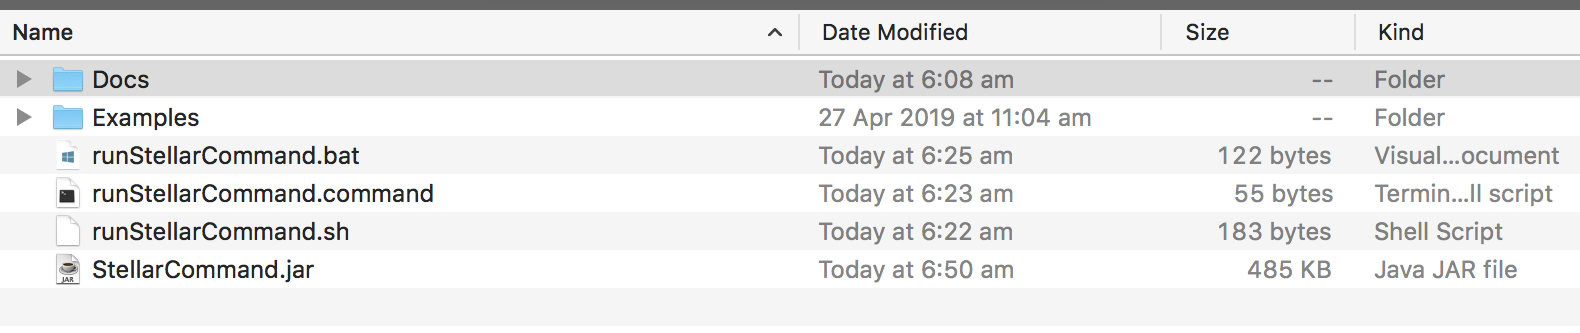
\includegraphics[width=1\columnwidth]{zipcontents}
	\caption{Stellar Command contents.}
	\label{fig:zipcontents}
\end{figure}

The \textit{Docs} folder contains the documentation files. The \textit{Examples} folder contains examples inside a \textit{HappyBrackets} project. The file \textit{StellarCommand.jar} is the Java archive that you need to include in your project if you are using it as a library. The remaining files are scripts for running in MacOS, Linux or Windows. Instructions for launching Stellar Command are in chapter~\ref{chap:launchosc} --
\emph{\titleref{chap:launchosc}}, with specifics on scripts in described in section ~\ref{sec:configscript} --
\emph{\titleref{sec:configscript}}.

\section{Setup Examples}\label{subsec:runningexamples} \index{Examples!HappyBrackets}
The examples for demonstrating Stellar Command are run using the HappyBrackets creative coding kit. In order to use the kit, you must install Java, IntelliJ and the HappyBrackets IntelliJ plugin. Instructions can be found at \url{https://github.com/orsjb/HappyBrackets/wiki/Getting-Started}.

Once you have installed HappyBrackets, open the Examples project by selecting \textit{Open Project} in IntelliJ (Figure~\ref{fig:openproject}) and then selecting the \textit{Examples} folder and pressing \textit{Open}, as shown in Figure~\ref{fig:selectproject}.

\begin{figure}[htbp]
	\centering
	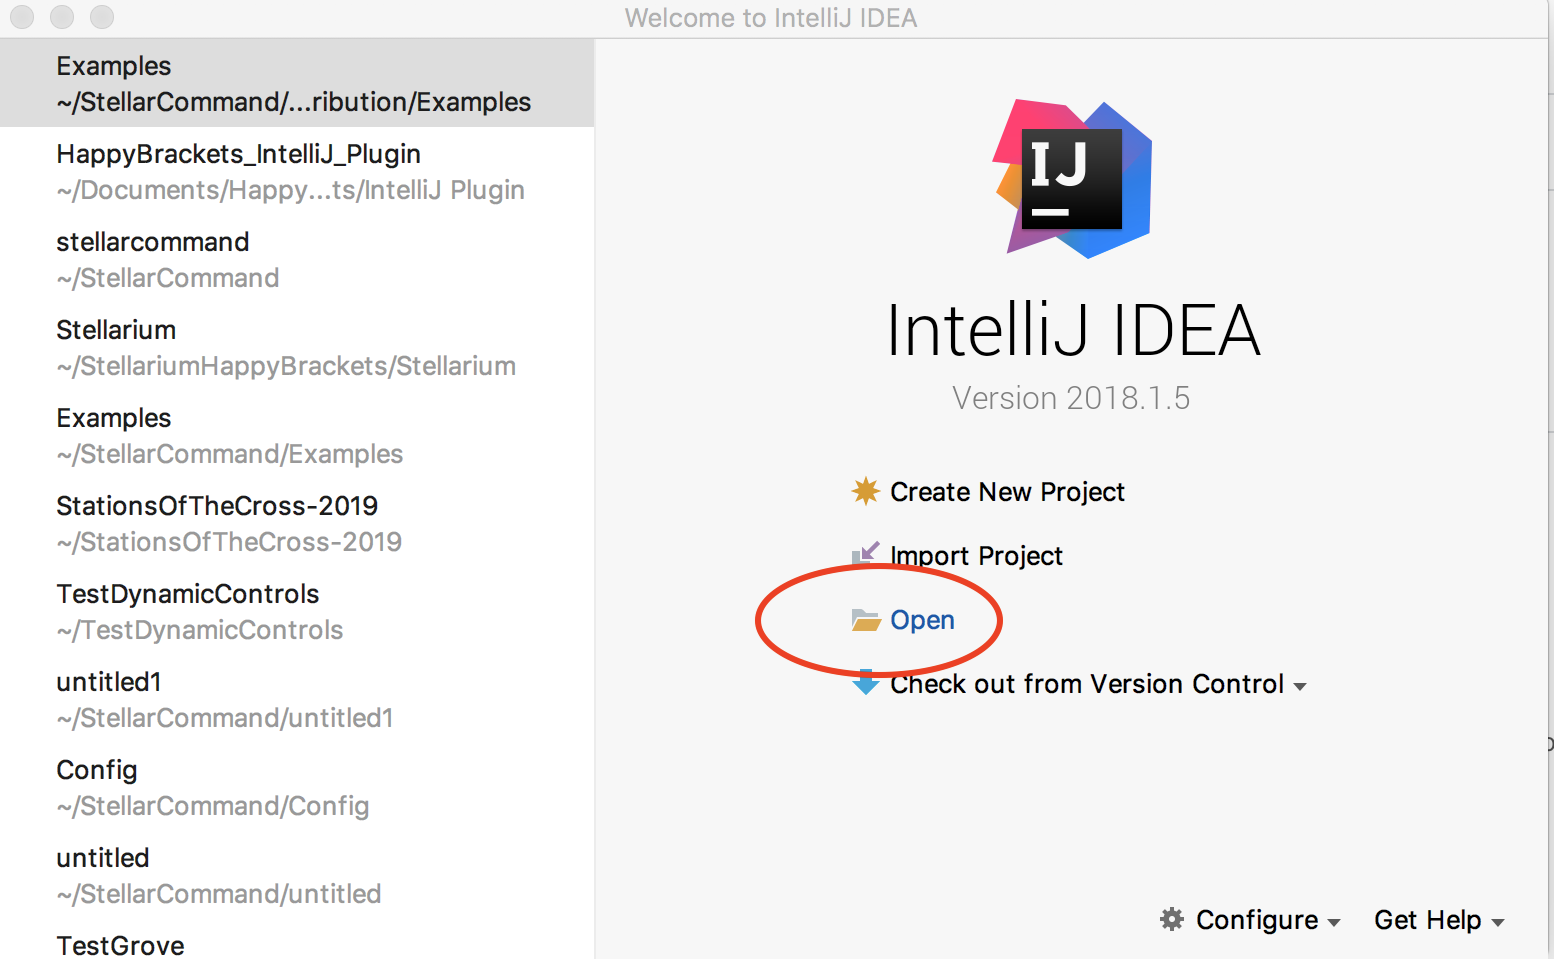
\includegraphics[width=1\columnwidth]{openproject}
	\caption{Select Open Project in IntelliJ}
	\label{fig:openproject}
\end{figure}

\begin{figure}[htbp]
	\centering
	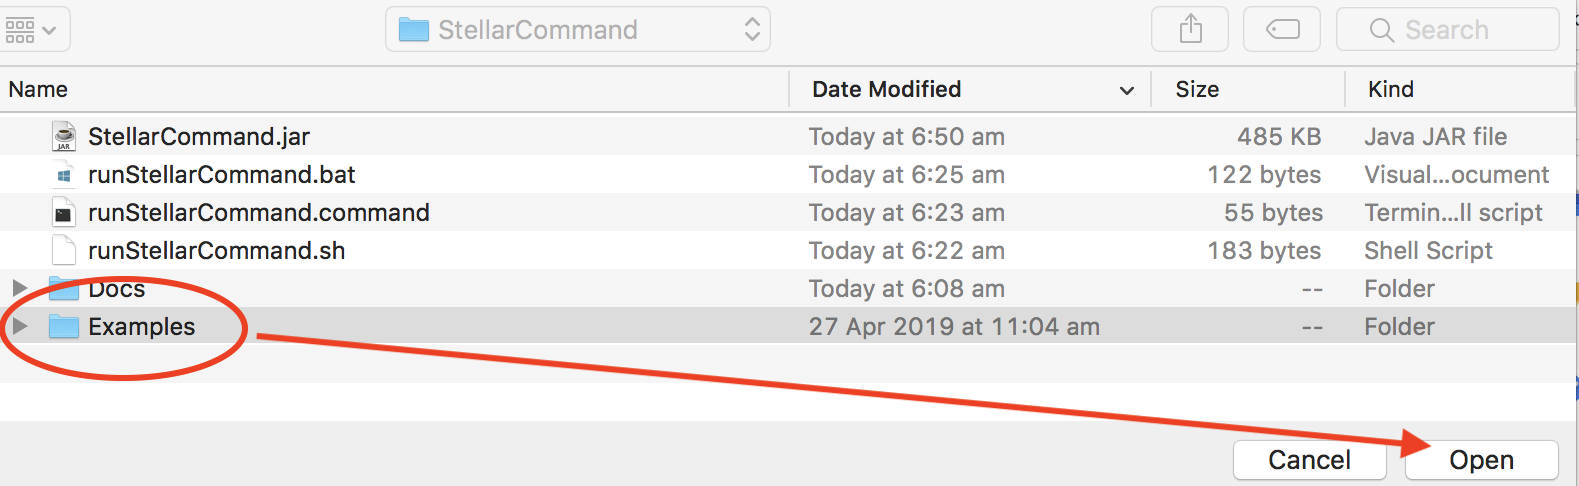
\includegraphics[width=1\columnwidth]{selectproject}
	\caption{Select Examples and press "Open"}
	\label{fig:selectproject}
\end{figure}

DO NOT enter into the \textit{Examples} folder as shown in Figure~\ref{fig:badopen} as this will not open the project. If you inadvertently get to this stage, press cancel and try again.. 

\begin{figure}[htbp]
	\centering
	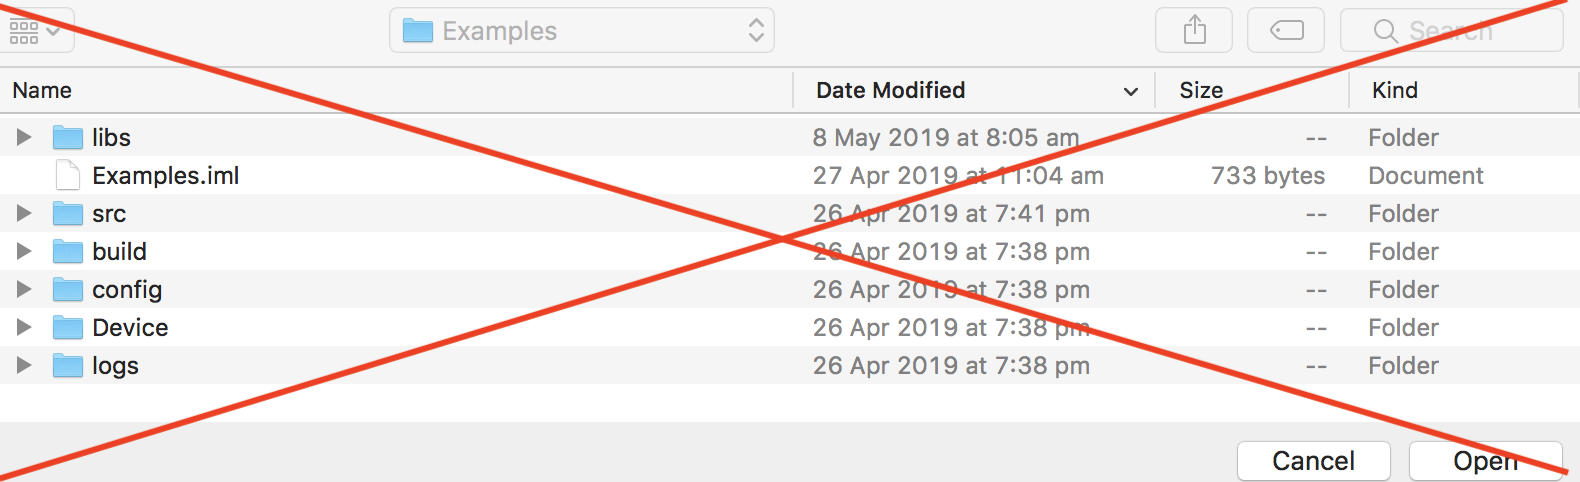
\includegraphics[width=1\columnwidth]{badopen}
	\caption{Incorrect attempt at opening Example Project}
	\label{fig:badopen}
\end{figure}






\chapter{Using Stellar Command with OSC} \label{chap:launchosc}
There are primarily two ways to use Stellar Command. The first is as a separate process that runs on the compute. The second method is to use Stellar Command as a library that you link to directly in your program. If you intend to use Stellar Command as a library, you can skip forward to chapter~\ref{chap:libraryosc} --
\emph{\titleref{chap:libraryosc}}.


\section{Launching Stellar Command}
makeidx{standalone}
\index{osc!clientport}
\index{osc!port|}
The Stellar Command module is instantiated by executing Java  with the name of the JAR file and the required program arguments that define communication, such as the network port to send OSC messages to, and the OSC address space.  For example, to start the StellarCommand module so it sends OSC messages on UDP port 1234  using an OSC address space of \texttt{/Stellar},\footnote{In this instance, the OSC client and Stellarium are on the same computer.} one would execute the following command:\\

\begin{syntax}

	java -jar StellarCommand.jar port=1234 osc=/Stellar  \\

\end{syntax}
\bigskip
   When the server starts, it will open the first available UDP port, and notify the client of this port. For example, if the command module opened port 4567, it will send an OSC message \texttt{/Stellar/osc 4567} to the client on the localhost. 
   
\begin{syntax}

	/Stellar/osc 4567  \\

\end{syntax}
\bigskip

Allowing the command module to find its own port number removes the probability of port clashes as each client furnishes the other with a valid port number for communicating without requiring configuration in the command module. It is, however, possible to request the Stellar Command module try certain ports by adding the argument \textit{tryport} \index{osc!tryport|(} with a comma separated list of ports. For example, the argument \texttt{tryport=3333,4444,5555} will cause Stellarium to sequentially try opening the ports listed, and if these all fail, will then open the first available port.\\
   
   \begin{syntax}

   	java -jar StellarCommand.jar port=1234 osc=/Stellar  tryport=3333,4444,5555\\

   \end{syntax}
   \bigskip
   
   The OSC client would receive the following OSC message:
   \begin{syntax}
   	/Stellar/osc 3333  \\
   \end{syntax}
   \bigskip
   
The OSC client and the Stellarium server do not have to be on the same physical computer as the Stellar Command module. For example Figure~\ref{fig:RemoteStellarium}, shows three OSC clients and a Stellarium server on a LAN, and a remote Stellarium server accessible from the internet through \textit{myserver.com}. 

\begin{figure}[htbp]
	\centering
	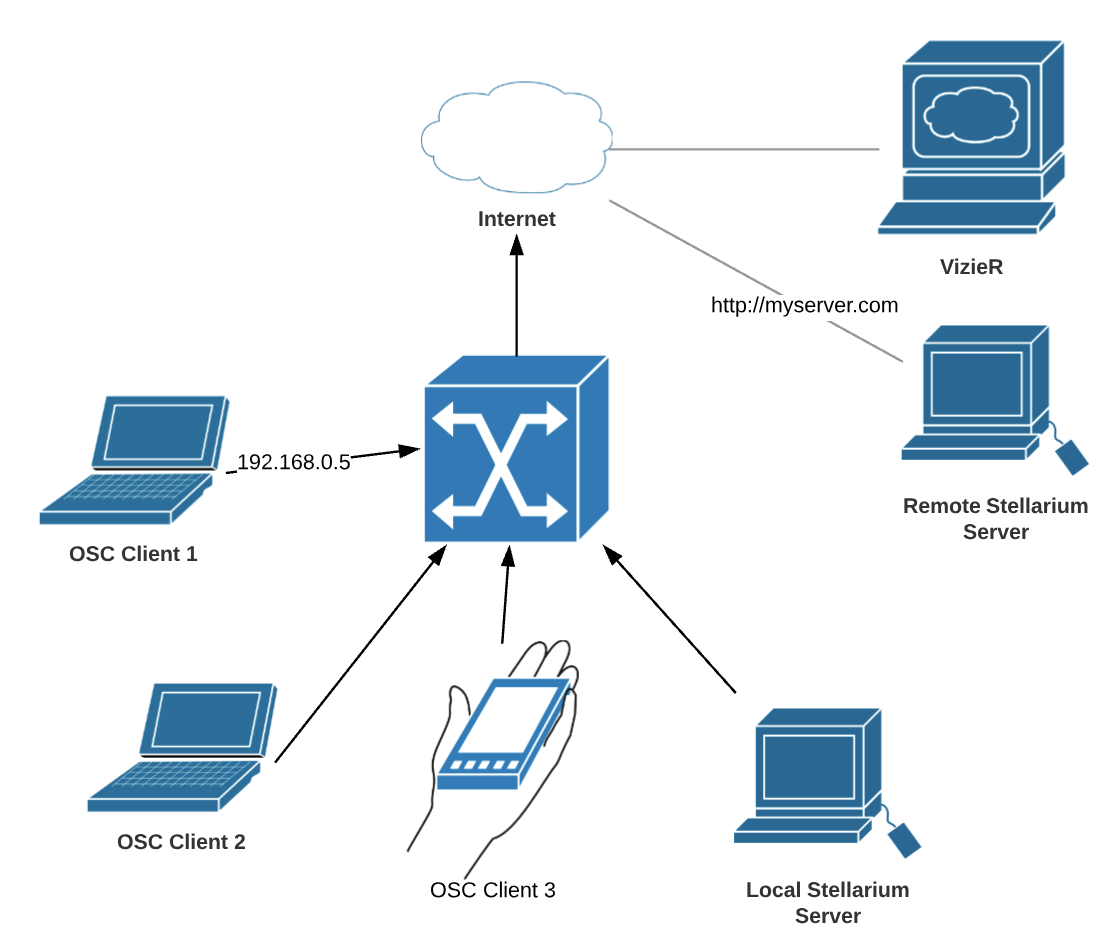
\includegraphics[width=1\columnwidth]{RemoteStellarium}
	\caption{Remote Stellarium and OSC Clients.}
	\label{fig:RemoteStellarium}
\end{figure}
\bigskip

Creating a connection between \textit{OSC Client 1} and \texttt{Remote Stellarium Server} is effected by adding adding the arguments \\\texttt{client=192.168.0.5} and \texttt{stellarium=http://myserver.com} to the command line.
This will cause the Stellar Command module to send OSC messages to ``192.168.0.5" and Stellarium commands to \textit{http://myserver.com} on HTP port 8090\footnote{The default Stellarium Remote Control port is 8090, however, this can be changed inside Stellarium. It is assumed that port forwarding when not using a local area network has been configured to send packages to the correct computer hosting Stellarium}, effectively acting as a proxy between the two.

 \begin{syntax}
	\medskip
	java -jar StellarCommand.jar port=1234 osc=/Stellar  {\char'134}\\client=192.168.0.5 stellarium=http://myserver.com\\
	\medskip
\end{syntax}
\bigskip

\section{Sending Commands to the Stellar Command Module}
You can provide instructions to Stellar Command in order to control Stellarium or to change the amount and type of data you want to receive. For example, you may want the Stellarium display to zoom in closer to a particular area of sky. You would do this by decreasing the field of view.\footnote{Section~\ref{subsec:fieldofview} --
	\emph{\titleref{subsec:fieldofview}} shows how to do this.} Likewise, you may want to reduce the amount of astronomical data you are receiving by adding a filter threshold so VizieR will only receive stars within a certain magnitude range. 

\subsection{poll}
Sometimes Stellar Command may already be started and configured to send and listen to the ports. You can easily find this out by sending the \textit{poll} command with no arguments, which will cause Stellarium to reply on the ports it is configured when started up.

 \begin{syntax}
	\medskip
	Stellar/poll
	\medskip
\end{syntax}

If you were sending OSC on the required port and your cleint was at the correct address, you would receive the following OSC message:
\begin{syntax}
	/Stellar/osc 3333  \\
\end{syntax}
\bigskip


\subsection{fieldOfView}\label{subsec:fieldofview}

In order to send a change in the field of view, send a message using the \textit{fieldOfView} in the namespace, followed by the field of view as a float argument. For example, to set the field of view to 60$^{\circ}$, you would send a message as follows:
 \begin{syntax}	
 	\medskip
	/Stellar/fieldOfView 60.0
	\medskip
 \end{syntax}
\bigskip

\subsection{moveLR}
You can make the Stellarium display move left or right by sending the command \textit{moveLR} followed by a floating point number indicating how far to move. A positive value will make it appear that the viewer is turning their head to the right, while a negative number will simulate moving to the left. To move to the right, send the following command:
  \begin{syntax}	
 	\medskip
 	/Stellar/moveLR 1.0
 	\medskip
 \end{syntax}
 \bigskip

\subsection{moveUD}
You can make the Stellarium display move up or rdown by sending the command \textit{moveUD} followed by a floating point number indicating how far to move. A positive value will make it appear that the viewer is turning their head up, while a negative number will look lower. To look towards the sky, send the following command:
\begin{syntax}	
	\medskip
	/Stellar/moveUD 1.0
	\medskip
\end{syntax}
\bigskip

\subsection{azimuth}
If you want to change the azimuth that you are looking at, use \textit{azimuth} in the namespace and add the azimuth as a float argument. For example, if you wanted to turn to the east, you would send a message as follows:
 \begin{syntax}	
	\medskip
	/Stellar/azimuth 90.0
	\medskip
\end{syntax}

\subsection{altitude}
If you want to change the altitude that you are looking at, use \textit{altitude} in the namespace and add the altitude as a float argument. For example, if you wanted to look 45$^{\circ}$ up, you would send a message as follows:
\begin{syntax}	
	\medskip
	/Stellar/altitude 45.0
	\medskip
\end{syntax}

\subsection{viewAltAz}
Setting the altitude and the azimuth at the same time is so commonplace that it has been made available as a single OSC message.
If you want to change the altitude that you are looking at, use \textit{viewAltAz} in the namespace and add the altitude and then the azimuth as float arguments. The two previous calls could have been done with the single command
\begin{syntax}	
	\medskip
	/Stellar/viewAltAz 45.0 90.0
	\medskip
\end{syntax}

\subsection{viewRADec}
You can move to the RA and Dec to the centre of the sky by using  \textit{viewRADec} in the namespace and send the RA and Dec as decimal degrees. If for example, you wanted to centralise  an RA of 95.98796$^{\circ}$  and Dec. of -52.69566$^{\circ}$  (this is the star Canopus), you would send the following OSC:
 \begin{syntax}	
 	\medskip
 	/Stellar/viewRADec 95.98796 -52.69566
 	\medskip
 \end{syntax}
 
 \subsection{View Object}
 You may want to select a particular named object in the sky, such as a star, planet or moon. You can do this by using the command \textit{viewObject} followed by the object name. For example, if you wanted to centre the planet Saturn, you would send the following OSC:
 
\begin{syntax}	
 	\medskip
 	 /Stellar/viewObject Saturn
 	\medskip
 \end{syntax}
 
 \subsection{viewerObservationPoint}
 You can change the latitude, longitude, altitude and planet you are setting as your observation point by using the \textit{viewerObservationPoint} command followed by the latitude, longitude, and altitude as float arguments, and the planet as a string.  For example, to set a latitude of 32$^{\circ}$, longitude of 151$^{\circ}$, and altitude of 21m from Saturn, you would send the following command:
 
 \begin{syntax}	
 	\medskip
 	/Stellar/viewerObservationPoint 32.0 151.0 21.0 Saturn
 	\medskip
 \end{syntax}
 
 
 \subsection{showGround }
 It is possible to hide the ground, enabling you to see stars and planets through the earth by sending the \textit{showGround } command, and an integer value of zero to hide the ground or non-zero to show it. To hide the ground, you would send the following OSC message:
 
  \begin{syntax}	
 	\medskip
 	/Stellar/showGround 0
 	\medskip
 \end{syntax}

 \subsection{showAtmosphere }
It is possible to hide the atmosphere, enabling you to see stars and planets during daylight hours by sending the \textit{showAtmosphere} command, and an integer value of zero to hide the atmosphere or non-zero to show it. To hide the atmosphere, you would send the following OSC message:

\begin{syntax}	
	\medskip
	/Stellar/showAtmosphere 0
	\medskip
\end{syntax}

 \subsection{showStarLabels }
It is possible to hide the star labels  by sending the \textit{showStarLabels} command, and an integer value of zero to hide the labels or non-zero to show it. To hide the labels, you would send the following OSC message:

\begin{syntax}	
	\medskip
	/Stellar/showStarLabels 0
	\medskip
\end{syntax}

 \subsection{showConstellationart }
It is possible to show or hide the constellation art by sending the \textit{showConstellationart} command, and an integer value of zero to hide the art or non-zero to show it. To show the constellation art, you would send the following OSC message:

\begin{syntax}	
	\medskip
	/Stellar/showConstellationart 1
	\medskip
\end{syntax}

\subsection{timeRate}
It is possible to change the simulated time rate on Stellarium by sending the \textit{timeRate} command followed by the new time rate in days per second as a float. If, for example, you set the time rate to zero, time would be still and the stars would not move through the sky. If, however, you set the time rate to 0.5, the display would simulate time running at one day every two seconds. You can also make time go in reverse by setting the time rate to a negative number. To set the display to simulate a day every two seconds, you would send the following:

\begin{syntax}	
	\medskip
	/Stellar/timeRate 0.5
	\medskip
\end{syntax}

\subsection{saveTable and loadTable}
Retrieving astronomical data from VizieR can sometimes take time, depending on your internet speed and the number of stars in the field of view requested. It is possible to save the current loaded VizieR table of stars to a file so you can use it even when there is no internet. To save the table, send the command \textit{saveTable} followed by the name of the file you want it saved to. You can then use the \textit{loadTable} command later to load the data and have Stellar Command send it to you.
To save the current table to the file "Acrux.txt", send the following command:
 
 \begin{syntax}	
 	\medskip
 	/Stellar/saveTable Acrux.txt
 	\medskip
 \end{syntax}

To load this table from file and have it send the data to you, send te following command:
 \begin{syntax}	
	\medskip
	/Stellar/loadTable Acrux.txt
	\medskip
\end{syntax}
\chapter{Decoding OSC Messages}
As stated in Section ~\ref{sec:launchcommand} --
\emph{\titleref{sec:launchcommand}}, OSC is received from Stellar Command on the port that Stellar Command is configured with alongside the OSC name space. If for example, you had launched Stellar command as follows:
\begin{syntax}
	\medskip
	java -jar StellarCommand.jar port=1234 osc=/Stellar  \\
	\medskip
\end{syntax}

You would receive all OSC messages from Stellar Command on port \textit{1234} with all messages prefixed with the namespace \textit{Stellar}. We will ignore the leading namespace in these instructions and assume that you will be filtering it.

\section{osc}
This should be the first message you receive from Stellar Command. The \textit{osc} name indicates the UDP port you need to send OSC messages to Stelar Command on.

\section{view}
The \textit{view} message will contain the following OSC arguments:
\begin{enumerate}
	\item float - Field of view. This is the field of view in decimal degrees. 
	\item float - the Right Ascension (RA) of the centre point of the display
	\item float - the Declination (Dec.) of the centre point of the display
\end{enumerate}
Consider the following received message:
\begin{syntax}
	/Stellar/view 20.0 96.49851 -52.682182  \\
\end{syntax}
\bigskip
This would indicate a 20 $^{\circ}$ field of view, RA of 96.49851$^{\circ}$ and Dec. of -52.682182$^{\circ}$.

\section{Star Values}
In many cases, sending astronomical data for all the stars within a certain radius a point would require create a message that would be too big for a single OSC packet. If we wanted to send astronomical data for say 1000 stars, we would need to send more than one packet. To accommodate this, Stellar Command will send multiple packets of data in bundles, with each packet containing OSC messages with  three distinct types of OSC messages - 1 x \textit{bundleCount} message, 1 x \textit{names} message and 0 or more \textit{values} messages. 

For example, one complete set of astronomical data might appear as follows:

\begin{syntax}
	Bundle 1 of N\\
	Star Column names\\
	Star Values \\
	Star Values \\
	Star Values \\
	...\\
	Star Values \\
	\\
	Bundle 2 of N\\
	Star Column names\\
	Star Values \\
	Star Values \\
	Star Values \\
	...\\
	Star Values \\
	
	....\\
	Bundle N of N\\
	Star Column names\\
	Star Values \\
	Star Values \\
	Star Values \\
	...\\
	Star Values \\
	
\end{syntax}

\subsection{bundleCount}
The \textit{bundleCount} message will contain the bundle number and the total number of bundles as arguments. The bundle number will be a zero based index, meaning that the first bundle will be bundle zero.For example, the bundleCount message for the first bundle of 15 bundles would appear as follows:

\begin{syntax}
	/Stellar/bundleCount 0 15
\end{syntax}
\bigskip

\subsection{names}
The names of the astronomical data columns is returned in the message names, with each OSC argument being the name of the  data. Stellar Command has configured VizieR to use the Hipparcos catalogue. The column of data returned are as follows: 

\begin{itemize}
	\item RArad (deg) -  Right Ascension in ICRS, Ep=1991.25 
	\item DErad (deg) -  Declination in ICRS, Ep=1991.25
	\item pmRA (mas/yr) -  Proper motion in Right Ascension
	\item pmDE (mas/yr) - Proper motion in Declination 
	\item Hpmag (mag) - Hipparcos magnitude
	\item B-V (mag) -  Colour index
\end{itemize}

\subsection{values}
Each bundle will return zero or more OSC messages that contain the data values that correlate to the column names in the \textit{names} message. Table~\ref{tab:vizierData} shows how the column names correlate to the astronomical data. Note that \textit{/Stellar} was removed from table example for brevity.

\begin{table}
	\centering
	\caption{Sample correlated column names and data}
	\begin{tabular}{|l|l|l|l|l|l|l|}  \hline
		\textbf{OSC Name}&\textbf{OSC arg}&\textbf{OSC arg}&\textbf{OSC arg}&\textbf{OSC arg}&\textbf{OSC arg}&\textbf{OSC arg} \\ \hline
		/names&RArad (deg)&DErad (deg)&pmRA (mas/yr)&pmDE (mas/yr)&Hpmag (mag) &B-V\\ \hline
		/values&000.111046 &-79.061831 &163.54  & -62.97  &8.7854  &0.778\\ \hline
		/values&001.002533 &-80.39506  & 55.39  & -18.26  &7.9968  &0.314\\ \hline
		/values&001.155615 &-81.345318  &1.05     &0.76  &9.1961 & 0.239\\ \hline
		/values&001.34229  &-79.253912  & 23.95    &66.32  &7.8761  &1.093\\ \hline
		/values&001.517384 &-84.09820 &  20.14     &1.37  &8.6327  &1.576\\ \hline
		/values&001.85792748 &-77.49416  & -2.06    &-9.80  &8.5621  &1.014\\ \hline
		
		\hline\end{tabular}
	\label{tab:vizierData}
\end{table} 

\section{viewerObservationPoint}
The \textit{viewerObservationPoint} message will contain information regarding the viewers location within the stellarium simulation. The OSC arguments returned are:
\begin{enumerate}
	\item float - latitude in degrees. 
	\item float -longitude in degrees
	\item float - altitude in metres
	\item string - planet  observer is viewing from
\end{enumerate}

For example, the following OSC message would indicate we are viewing from a latitude of 15.824176 South, longitude of 70.520546 East, 930m high from Earth.

\begin{syntax}
	/Stellar/viewerObservationPoint -15.824176 70.520546 930.0 Earth
\end{syntax}

\section{time}
The \textit{time} message indicates the simulated time being displayed on stellarium. The arguments in the OSC message if we were viewing at midday of 8 June 2019 in Sydney simulating a normal procession of time, would be are as follows:
\begin{enumerate}
	\item string - UTC as ISO formatted String. Eg, .2019-06-08T02:00:00.000Z
	\item string - Local time as a string eg. 2019-06-08T12:00:00.000
	\item float - GMT time shift in Julian days. eg 0.41666666
	\item float - the current time rate in Julian days 1.1574074E-5
\end{enumerate}

Note that time rate is actually a double precision number, however, OSC does not natively support double values. 1.1574074E-5 is approximately the number of days in a second.

\chapter{OSC Examples}\label{chap:oscexamples}\index{OSC Examples}
The examples provided use the HappyBrackets creative coding toolkit and are coded in Java. For details on installing HappyBrackets, see section \ref{subsec:runningexamples} --
\emph{\titleref{subsec:runningexamples}}

The examples are configured to use port 1234 as the port you will receive OSC from Stellar Command. Additionally, it is configured to have Stellar Command listend on ports 3333, 4444 or 5555. These are the same configuration setting used in the description in section \ref{sec:launchcommand} --
\emph{\titleref{sec:launchcommand}}.

\section{Example Source Location}\index{OSC Examples!Example files location}

The source files for the OSC examples are under the \textit{src/stellarcommandexamples/osc} folder, as shown in 
Figure~\ref{fig:oscexamplefolder}.

\begin{figure}[htbp]
	\centering
	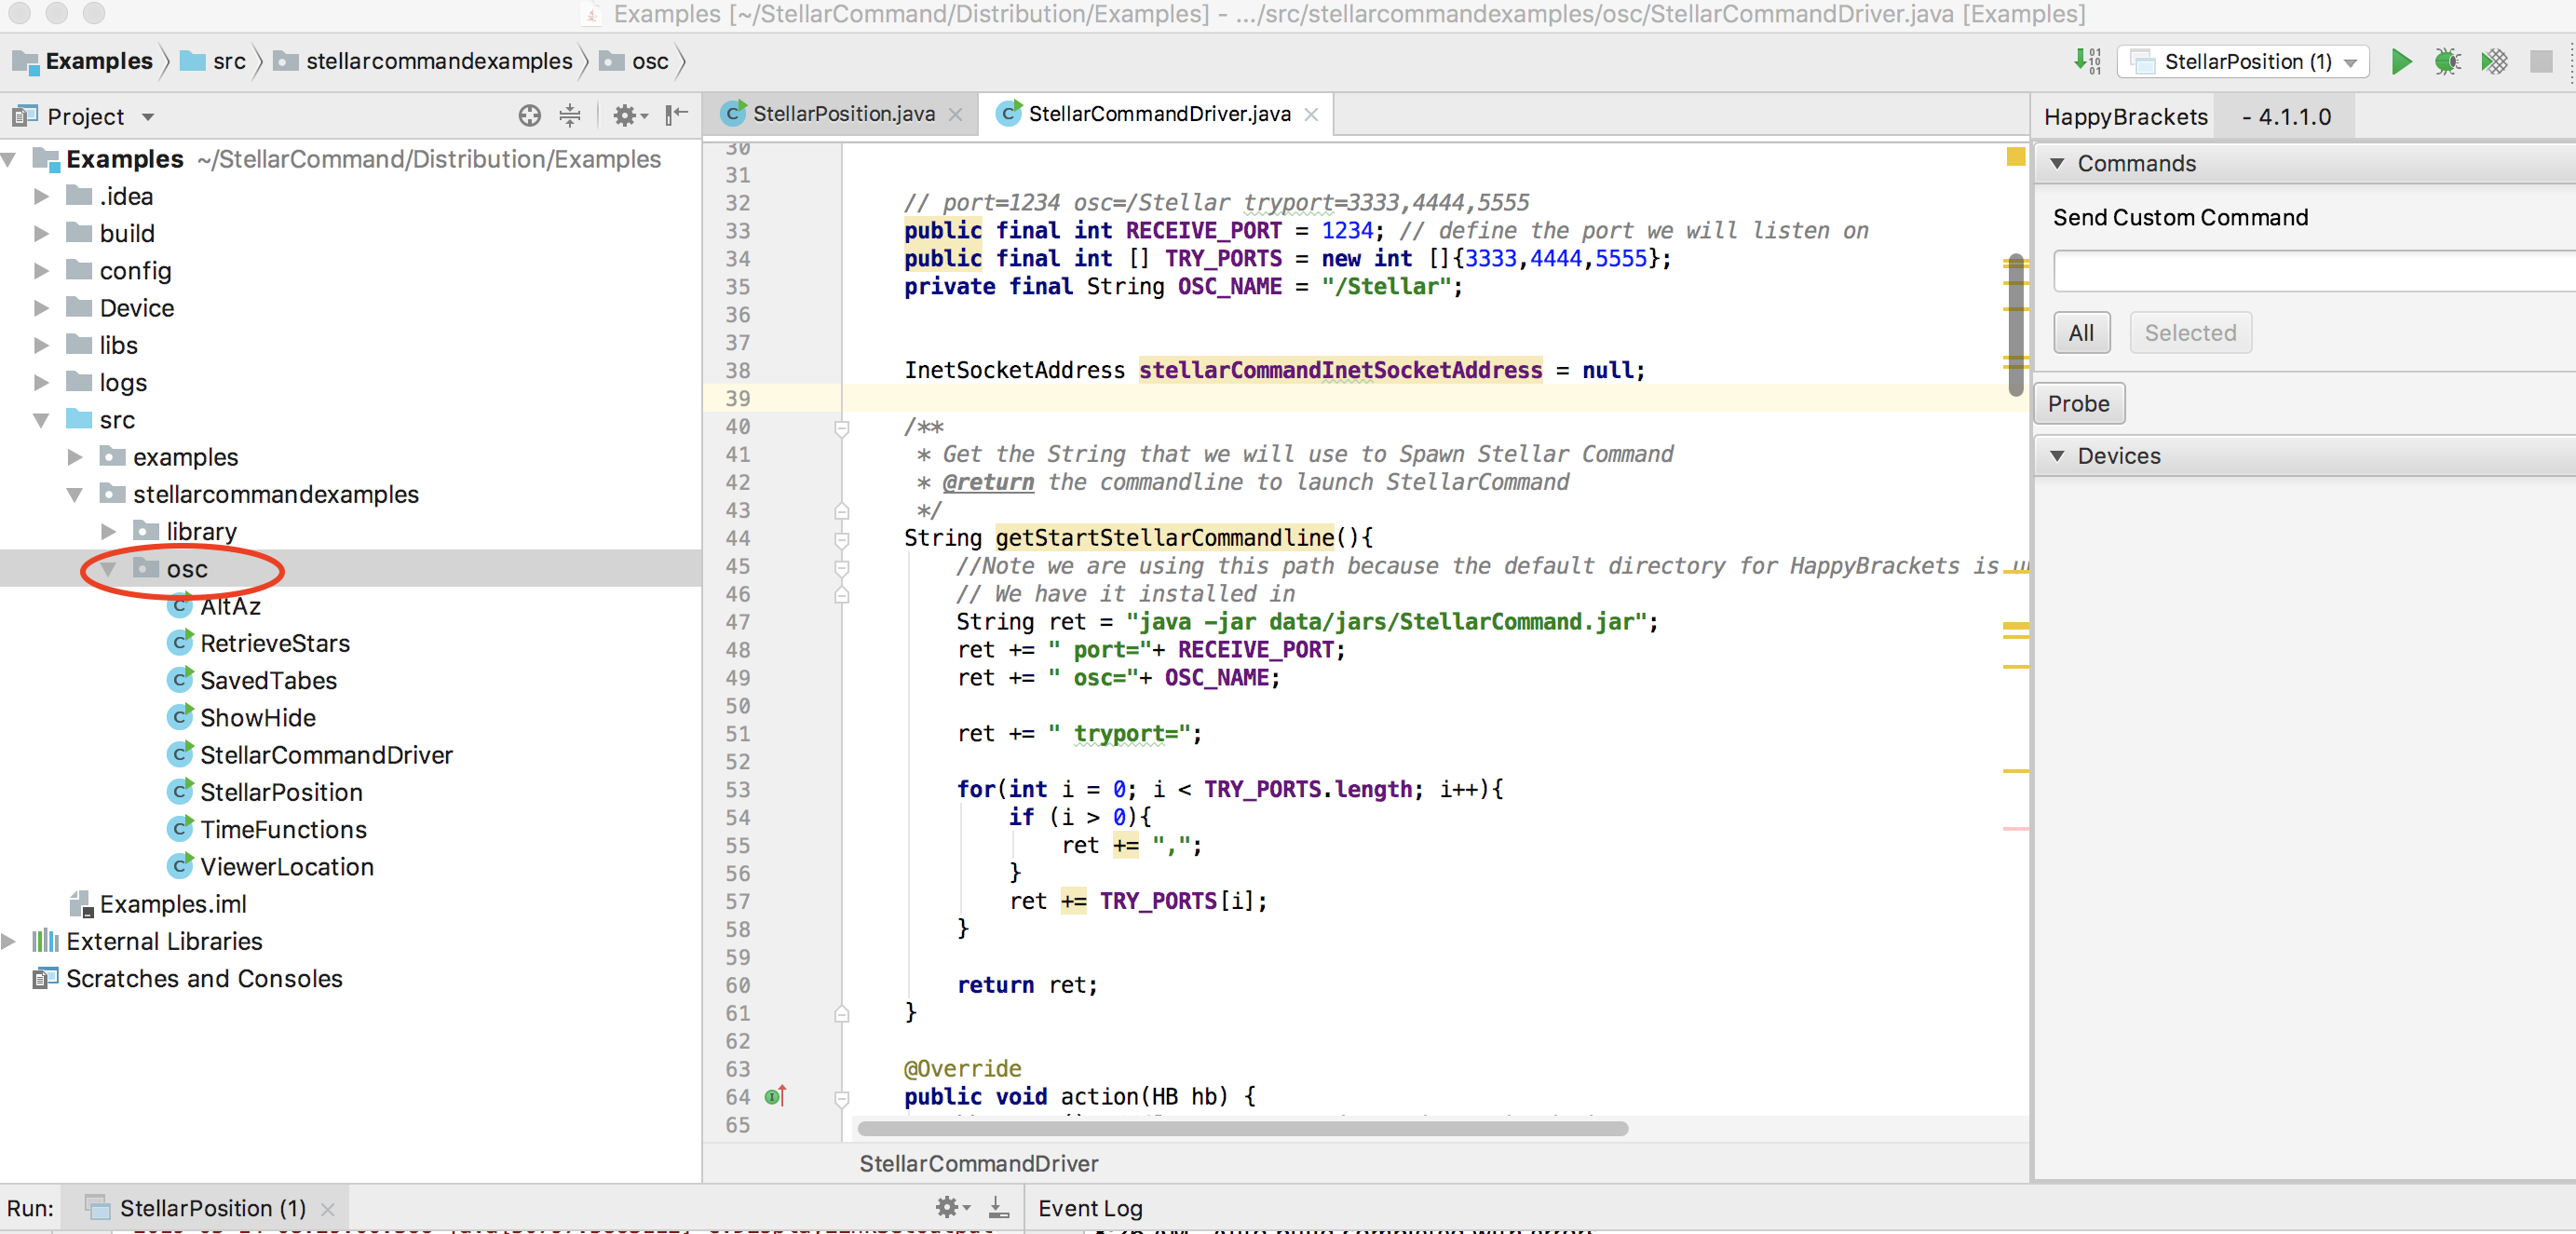
\includegraphics[width=1\columnwidth]{oscexamplefolder}
	\caption{OSC examples folder.}
	\label{fig:oscexamplefolder}
\end{figure}
\bigskip




\chapter{Using Stellar Command as a Java Library} \label{chap:libraryosc}
This chapter details how to use Stellar Command as a library that you call directly from within your programming environment.
If you intend to use Stellar Command as a standalone server application and communicate to it with Open Sound Control Messages through your preferred music package---such as Max MSP, SuperCollider or PD---you can skip back to chapter~\ref{chap:launchosc} --
\emph{\titleref{chap:launchosc}}.

The Stellar Command Library is a Java Archive that provides a far more efficient method of controlling Stellarium and accessing the data because the structures can be accessed directly without having to convert them to OSC. In some cases, converting values to OSC  can result in  data loss when the parameter is a double. Similarly, if a VizieR query contains many thousands of rows of data, these do not need to be encoded into OSC, parsed, and then decoded again. Furthermore, you can easily do efficient functions such as sorting and obtaining altitude and azimuth based on observer location and date and time directly.

The three main packages include in the Jar are Stellarium Control (packed as\textit{stellarium}), VizieR query (packaged \textit{vizier}), and complex data conversion (packaged \textit{stellarstructures}).

\section{stellarium}
The simplest way to access Stellarium is through the \textit{stellarium} package. The package contains various classes to simplify communication with Stellarium. Rather than detailing every function, which you can easily access through the online documentation, the class names and their basic functions will be outlined.
\subsection{StellariumSlave}

\textit{StellariumSlave} is the class that does the REST communication to Stellarium and provides a common access point. The class contains a synchronised threaded model that enables API calls to Stellarium to complete asynchronously. If, for example, you wanted to set the azimuth of the Stellarium display, you would call \textit{setAzimuth} with the number of degrees and your function would return immediately. The StellariumSlave class would then send the API request to Stellarium in a separate thread. This prevents the calling application form having to wait for Stellarium to process the request, which can often take over 100ms. 
StellariumSlave provides the facility to poll Stellarium for changes and provides \textit{StellariumViewListener} interfaces for classes \textit{StellariumView, StellariumLocation} and \textit{StellariumTime}.

\subsection{StellariumView}
StellariumView contains properties about the display of Stellarium. These include the field of view, and the RaDec. RaDec are collated into a single class, as detailed in section ~\ref{sec:RaDec} --
\emph{\titleref{sec:RaDec}}. 

\subsection{StellariumLocation}
StellariumLocation contains information about the simulated location of the viewer in Stellarium. You can access parameters including latitude, longitude, altitude, planet and landscape.

\subsection{StellariumTime}
StellariumTime provides access to the time parameters of the Stellarium.  These include UTC time, local date time and GMT time shift based on the viewer location, the Julian day, and the time rate that Stellarium is simulating.

\subsection{StellariumProperty}
The \textit{StellariumProperty} has properties including the ability to show atmosphere, ground, star labels and constellation art. This is very much in progress and more properties will; be made accessible in time as the need arises.

\section{vizier}
The vizier packages provides the interface to  VizieR database of astronomical catalogues. 
\subsection{VizierQuery}
The \textit{VizierQuery} class is where you are able to define the catalogue you want to use, outputs that you require, and any filters that you want to apply. You cn then perform a read which will provide the astronomical data matching the query as text. This data can be reinterpreted using functions from the \textit{stellarstructures} package, detailed in   section ~\ref{sec:stellarstructures} --
\emph{\titleref{sec:stellarstructures}}. 

The default catalogue used is catalogue used is I/311/hip2 - Hipparcos, the New Reduction (van Leeuwen, 2007). The default outputs provided are:

\begin{itemize}
	\item RArad (deg) -  Right Ascension in ICRS, Ep=1991.25 
	\item DErad (deg) -  Declination in ICRS, Ep=1991.25
	\item pmRA (mas/yr) -  Proper motion in Right Ascension
	\item pmDE (mas/yr) - Proper motion in Declination 
	\item Hpmag (mag) - Hipparcos magnitude
	\item B-V (mag) -  Colour index
\end{itemize}

 \subsection{StellarDataTable}
\textit{StellarDataTable} performs analysis and conversion of VizieR data   and stores the data into a table structure. The StellarDataTable contains the names of the columns as well as a list of \textit{StellarDataRow} items that contain the astronomical data values.

\subsection{StellarDataRow}
A StellarDataRow contains astronomical data values for one star. The list of values match the column names in the StellarDataTable.

\subsection{StellarFilteredTable}
\textit{StellarFilteredTable} is a class for sorting a StellarDataTable.

 \subsection{FilteredData}
The \textit{FilteredData} class is a utility for sorting StellarDataRow items based on AltAz

\subsection{MagnitudeSort}
the \textit{MagnitudeSort} class is a utility for sorting StellarDataRow items based on magnitude


\section{stellarstructures} \label{sec:stellarstructures}
The following classes provide basic encapsulation and some functions on data.

\subsection{AltAz}
Contains a combination of altitude and azimuth as a single structure;

\subsection{RaDec}\label{sec:RaDec}
Contains the Right Ascension (RA) and the Declination (Dec.) as a single structure. RA is stored as decimal degrees rather than as hours, minutes and seconds.

\subsection{ObservationalPoint}
The \textit{ObservationalPoint} contains information about the UTC date / time, latitude and longitude of a particular point. This information is often required for performing other functions such as converting the RADec of a star to AltAz.

\subsection{StellarConversions]}
 The \textit{StellarConversions} is a utility class used for performing functions including converting RaDec to AltAz and converting Stellarium's three dimensional spherical points to RaDec.
 



	
\bibliography{StellarCommandManual} 
	
\printindex

\end{document}